	% !TeX encoding = UTF-8
% !TeX program = pdflatex
\documentclass[binding=0.6cm,LaM]{sapthesis}
\usepackage[utf8]{inputenx}
\usepackage{lscape} 

\usepackage{listings}
\usepackage{color}

\definecolor{dkgreen}{rgb}{0,0.6,0}
\definecolor{gray}{rgb}{0.5,0.5,0.5}
\definecolor{mauve}{rgb}{0.58,0,0.82}

\lstset{frame=tb,
  language=Java,
  aboveskip=3mm,
  belowskip=3mm,
  showstringspaces=false,
  columns=flexible,
  basicstyle={\small\ttfamily},
  numbers=none,
  numberstyle=\tiny\color{gray},
  keywordstyle=\color{blue},
  commentstyle=\color{dkgreen},
  stringstyle=\color{mauve},
  breaklines=true,
  breakatwhitespace=true,
  tabsize=3
}

\usepackage{hyperref}
\hypersetup{pdftitle={Thesis},pdfauthor={Danilo Bernardini}}
\title{Design, development and evaluation of a \\framework for recording and synchronizing \\experiences in VR with physiological signals}
\author{Danilo Bernardini}
\IDnumber{1544247}
\course{Engineering in Computer Science}
\courseorganizer{Faculty of Information Engineering, Informatics and Statistics}
\AcademicYear{2017/2018}
\examdate{20 July 2018}
\examiner{M. Schaerf}
\examiner{S. Bonomi}
\examiner{G. Grisetti}
\examiner{M. Mecella}
\examiner{D. C. D’Elia}
\examiner{D. Lembo}
\examiner{R. Rosati}
\copyyear{2018}
\advisor{Prof. Massimo Mecella}
\coadvisor{Prof. Maurizio Caon}
\authoremail{danilo.bernardini93@gmail.com}
\begin{document}
\frontmatter
\maketitle

\begin{acknowledgments} 
jsnib

\end{acknowledgments}

\tableofcontents
\mainmatter
\chapter{Introduction}



\chapter{Project concept and technologies}

This chapter introduces the project idea and the concepts behind it, starting from the use of VR combined with physiological signals and going towards use cases and project requirements. After this, involved technologies - virtual reality and physiological sensors - are illustrated in details and current state of the art is presented, including the available devices on the market. Finally, the last section is about the specific technologies used in this project.

\section{VR and physiological signals}
Virtual reality is a powerful tool not only for commercial use, but also for research. Since the beginning of its lifetime, in fact, people started to think that it could have been a good environment to test and study certain phenomenons, especially concerning human body and behavior. From the first VR basic prototypes to the advanced systems of these last years, researchers have conducted lost of experiments about people reactions and emotions with VR making use of physiological signals. The reason why virtual reality is so appropriate and useful for research is that it can simulate real situations, so it gives researchers countless opportunities: they can recreate real world environments, test new kinds of interaction, make people relive specific scenes, and so on. 

As mentioned above, for many years there have been several examples of studies about VR with the use of physiological signals. An early research paper dealing with this subject was the one about fear of flying written by Wiederhold and others and published in 1998 \cite{wiederhold1998fear}. The authors wanted to test if there are significant physiological differences between people who are afraid of flying and people who are not. In order to accomplish that, they studied the body responses of two groups of people, one suffering from a fear of flying and the other one not, while experiencing a virtual reality flight. They measured heart rate, peripheral skin temperature, respiration rate, sweat gland activity and brain wave activity. The results of the experiment were successful and they could conclude that there exist significant differences between these two groups of people. In addition, the authors also succeeded in reducing arousal of people with fear of flying making them experience the simulation for several times. 

The following year another research paper about VR and physiological signals was published by Cobb and others \cite{cobb1999virtual}. This was one of the first investigations about VR sickness (see \ref{sec:measures}): the authors examined effects and symptoms of virtual reality on people using several methodologies, including physiological parameters.

These examples are part of the several research studies conducted to analyze or treat specific phobias and diseases. More recent ones are, for example, those by Kuriakose and Lahiri \cite{kuriakose2015understanding} and by Seinfeld and others \cite{seinfeld2016influence}, published in 2015 and 2016, respectively. Both are about anxiety: the former aims at measuring anxiety level in adolescents with autism using physiological signals while being in VR, the latter examines the influence of music on anxiety induced by fear of heights in VR. 

Finally, we can include in this list a paper about the hand illusion in VR with temperature monitoring by Llobera and others \cite{llobera2013relationship} and one about reduction of pain and anxiety in dental procedures using VR distractions \cite{wiederhold2014clinical}.

\section{Idea and requirements}
There are many experiments and studies using virtual reality that also include physiological signals; the previous section presented some of them showing that VR applications are limitless and that using physiology with it can lead to important results.
There is a common aspect in all these kind of studies: if the researchers want to collect physiological data during a virtual reality experience, they need to set up everything. This means to find a way to follow the experiment, to see what the participant sees in VR, to store data and to be able to analyze it. All these things are possible only if the collected data - VR video, physiological signals and other available sources - are synchronized. This process implies a lot of effort from the researchers because they have to figure out how to design and realize it, wasting time they could invest in the actual research.

This leads to the basic motivation behind this thesis project: designing and implementing a framework for recording and synchronizing experiences in VR with physiological signals. The framework would be a useful tool for whoever wants to physiologically analyze a certain phenomenon in VR. Having a ready-to-use test environment would allow to save time and focus on the actual experiment; the only required thing is to build the virtual scene, everything else is done by the framework.

\subsection{Use cases}
The project requirements come from use cases. We can imagine two main cases that cover the two different parts of the application usage:

\begin{enumerate}

\item examiner wants to see in real-time and to record what the participant sees and how the body behaves;

\item examiner wants to replay a previously recorded session.

\end{enumerate}

Let us analyze these points one by one in order to fully understand what the system should do. After a brief description, for each use case is presented a diagram followed by the list of steps required to arrive to the goal, including the extensions.

\begin{enumerate}

\item Since the framework is designed for conducting VR researches with physiological signals, who conducts the experiment should be able to see what the participant sees in the virtual world in real-time and how the body reacts to the experience. 
In addition to this, the examiner should be able to record the whole session including all the signals and streams he has. This leads to an extension of the case, named \textit{Record session}, which can be executed only after the examiner is able to see everything correctly.
Once recorded, everything can be synchronized in order to be easily accessible and analyzable in the future. This brings the \textit{Record session} case to be extend in turn. 
The use case description assumes that the participant is ready, with all the physiological sensors attached to his body and the VR headset correctly placed.

\begin{figure}[h]
\centering
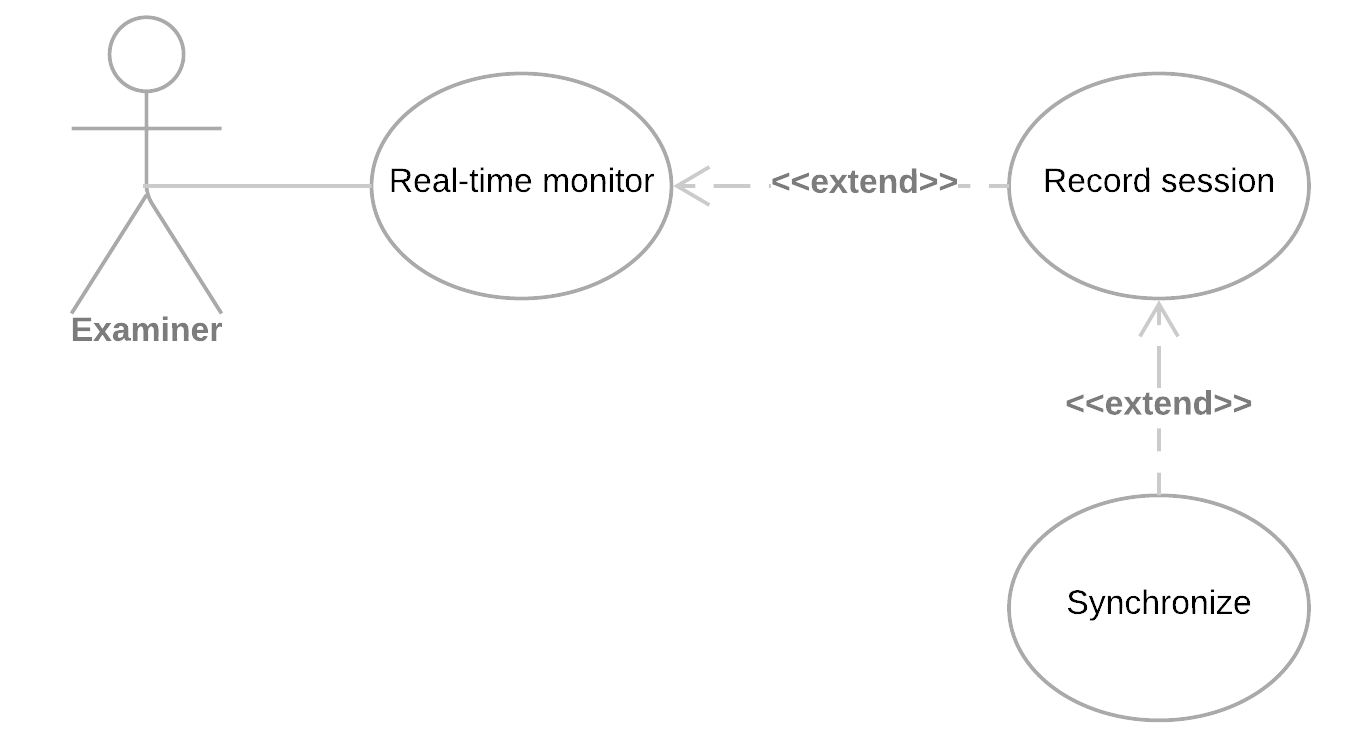
\includegraphics[scale=.24]{images/use_case_1}
\caption{\textit{Real-time monitor} case diagram}
\end{figure}

%\renewcommand{\arraystretch}{1.5}
\begin{center}
\begin{tabular}{| l | l |}
  \hline			
  Name & Real-time monitor \\
  \hline
  Initiator & Examiner \\
  \hline
  Goal & Monitor the session in real-time \\
  \hline  
\end{tabular}

\vspace{.5cm}

%\renewcommand{\arraystretch}{1}
\begin{tabular}{ l }
\textbf{Main success scenario} \\
1. Examiner runs the application\\
2. Examiner sets up the sensors in the application \\
3. Application displays sensors, VR and camera streams \\
4. Examiner sees everything in real-time \\

\vspace{0.1cm}\\

\textbf{Extensions} \\
4. Examiner wants to record the session\\
\quad a. Examiner starts a new recording \\
\quad b. VR, camera and sensors streams are stored \\
\quad c. Examiner stops the recording \\

4c. Examiner wants to synchronize the session\\
\quad a. Examiner starts the synchronization \\
\quad b. Synchronization completes \\

\end{tabular}

\end{center}

\item The examiner should have the possibility to offline replay a previously recorded session, being able to see everything as it was during the real-time monitoring. In this replay mode there should be the possibility to find key moments in which some relevant event happened. Since the session sources are synchronized, this task should be easy. The examiner should be able to tag these events placing markers on them: these would allow a simple navigation on the session and would also be very useful for analysis.

\begin{figure}[h]
\centering
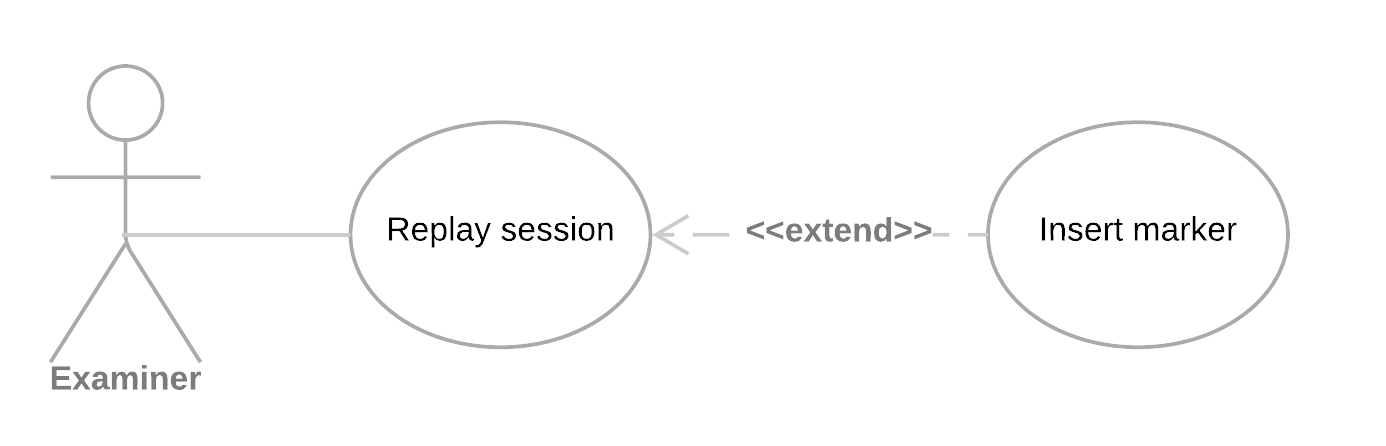
\includegraphics[scale=.257]{images/use_case_2}
\caption{\textit{Record session} case diagram}
\end{figure}

%\renewcommand{\arraystretch}{1.5}
\begin{center}
\begin{tabular}{| l | l |}
  \hline			
  Name & Replay session \\
  \hline
  Initiator & Examiner \\
  \hline
  Goal & Replay a prerecorded session \\
  \hline  
\end{tabular}

\vspace{.5cm}

%\renewcommand{\arraystretch}{1}
\begin{tabular}{ l }
\textbf{Main success scenario} \\
1. Examiner runs the application\\
2. Examiner selects the "replay" mode\\
3. Examiner opens one of the directories containing a previous recorded session \\
4. Examiner plays the session \\

\vspace{0.1cm}\\

\textbf{Extensions} \\
4. Examiner wants to insert one or more marker\\
\quad a. Examiner finds the moments he wants to mark \\
\quad b. Examiner inserts the marker and assigns it a label \\
\end{tabular}

\end{center}


\end{enumerate}

The whole UML Use Case Diagram is represented in figure 3.3. 

\begin{figure}[h]
\centering
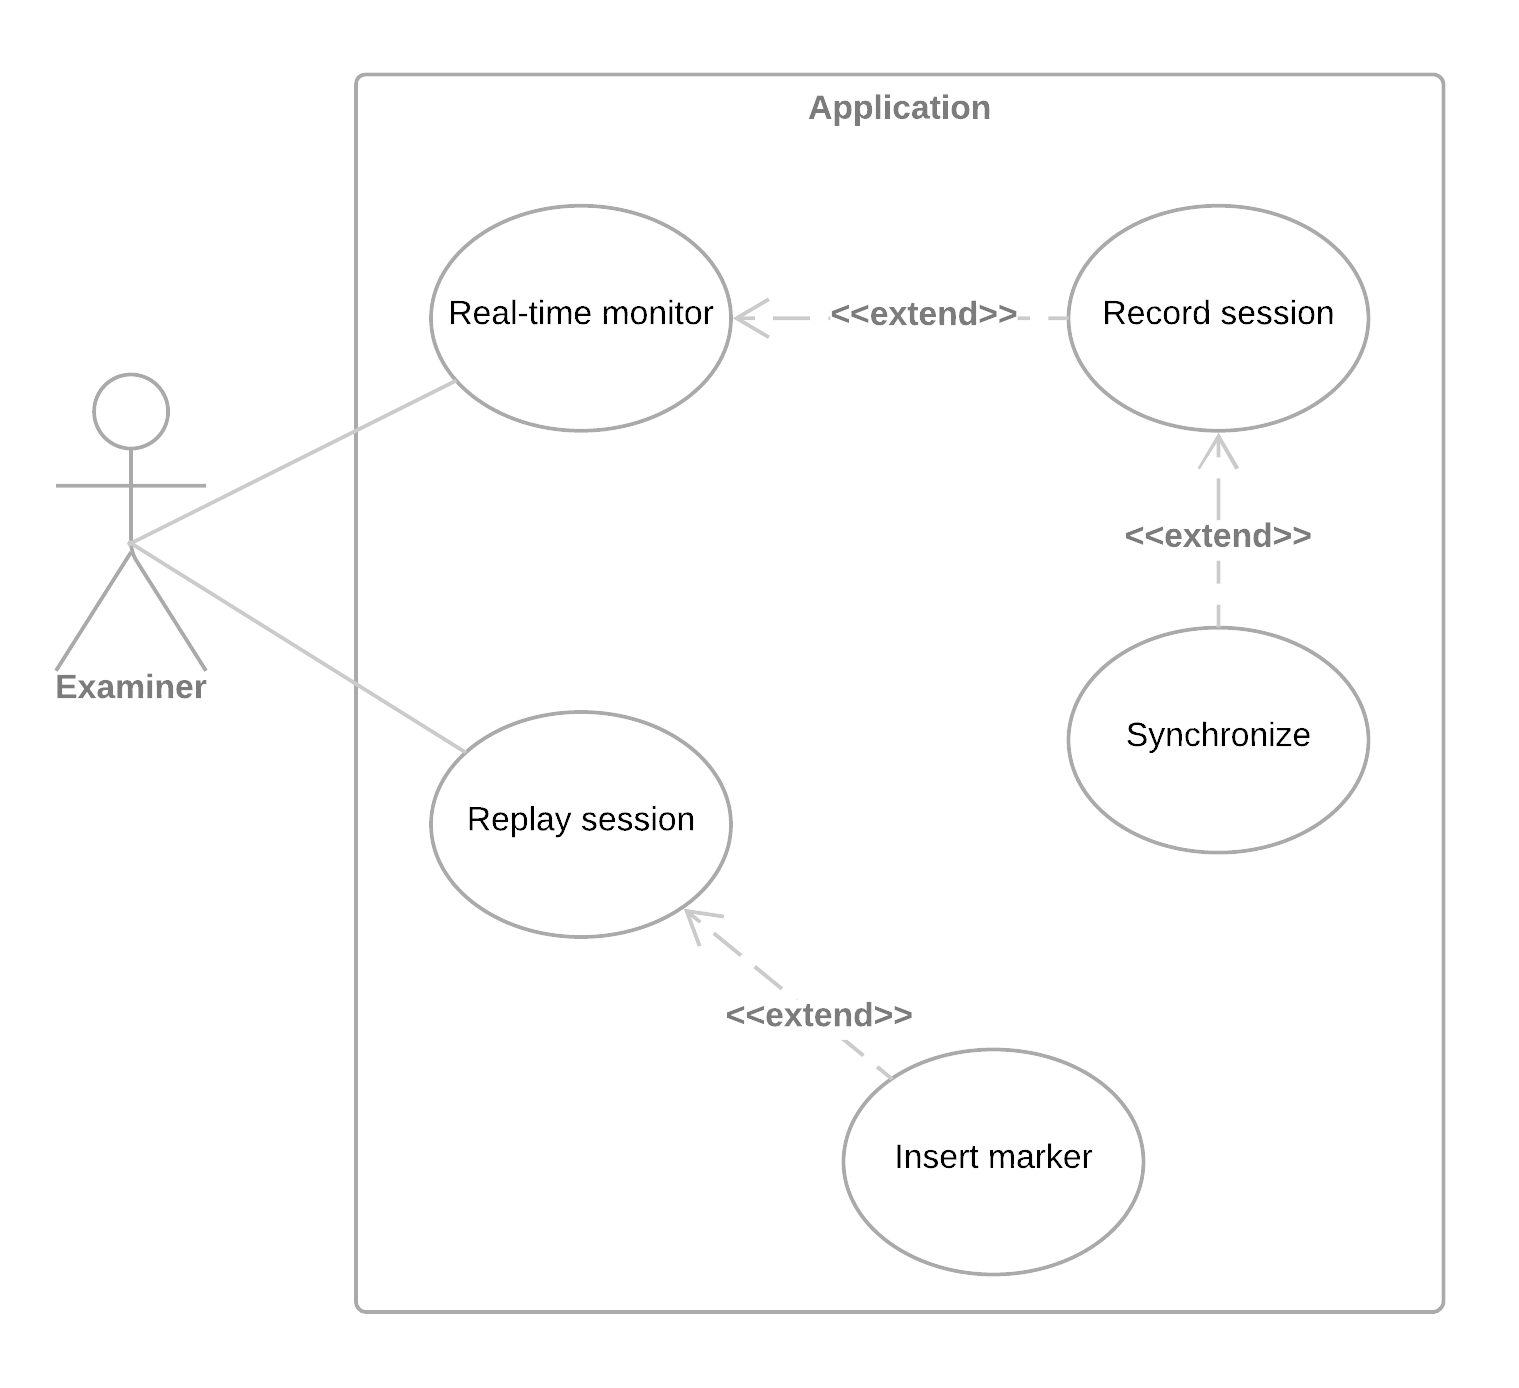
\includegraphics[scale=.257]{images/use_case}
\caption{Global Use Case Diagram}
\end{figure}


\subsection{Requirements}
This section is about the requirements for the project, which result from the above use cases and from some other considerations. 

The system should allow to monitor a virtual reality experience while some sensors collect the participant's physiological signals. It would be reasonable to include in the system a camera that films the participant during the experience. This would make it possible to also have an external view on the user, being able to monitor his physical reactions to events. Examiners can see if the participant moves, rotates his body, is not stable, or has any other kind of reaction in response to a virtual stimulus.

Moreover, system structure and usability should not be hard, considering that the potential users will not be engineers or computer science experts. These people, in fact, will reasonably be scientist, doctors or researchers that need to test and analyze something in VR. 

The system should allow to to start a new real-time monitoring session which shows what the participant sees in VR, the camera source filming him and his physiological signals. During this "live" session, the examiner should be able to start a new recording: this will store the streams from VR, camera and sensors. At the end of the experiment the examiner should stop the recording and the various data need to be automatically synchronized. Alongside with the real-time mode, the system should have an "offline" part that allows to replay a previously recorded session. This mode should provide classical playback controls such as play, pause and stop, as well as timeline navigation to quickly skip to a specific frame. Since everything is already synchronized, in this modality the examiner can easily track every moment of the experiment; if there are relevant events it is worth to emphasize, the system should allow to place markers on them. 
Finally, the stored files (VR video, camera video and sensors data) should remain independent from each other, i.e. they should still be accessible from external programs after the synchronization and markers insertion.

\section{Virtual Reality}
Virtual Reality (VR) is a technology that aims to allow a user to experience a computer-generated simulated environment. It commonly consists of a visual experience, but it can also include audio, haptic, touch and other feedback devices. 

Visual devices are usually VR headsets, head-mounted displays (HMD) with two screens - one per eye - that immerse the user in a virtual world simulating the real one. While wearing the headset, the user can look around rotating his head, move in the environment or interact with virtual objects using controllers, and perceive other senses through ad-hoc devices.

The above systems are usually computer-based, i.e. they are physically connected to the computer, so the applications run here and the visual output is transmitted to the headset display.
Another kind of solution is the one that uses the smartphone: in this case the headset is just a case that holds the device, the whole computation takes place in the smartphone and thus the applications are much simpler and less realistic compared to the computer-based ones (see \ref{sec:vrheadsets}).
	
\subsection{VR spread}
Virtual reality idea is not something new, there have been basic examples of it since the 1960s. The first head-mounted display system was the \textit{Sword of Damocles} \cite{sutherland1968head} created in 1968 by computer scientist Ivan Sutherland and his student Bob Sproull: the graphics were very primitive and consisted only of wireframe rooms, but the device was able to change the showed perspective according to the user head position. Its name comes from its appearance: the whole system was too heavy to be worn by a person so it was attached to the ceiling, suspended on the user's head.

In the next years different VR systems were developed, most of the times for the videogames industry. Examples can be found in some \textit{SEGA} and \textit{Nintendo} products. 

The main reason why VR is exploded in the last few years is that technology is now powerful enough to support advanced computation and to give users really immersive experiences. Until a few years ago VR solutions could not satisfy \textit{immersion} requirements (see section \ref{sec:measures}): graphics were not good enough and they had low refresh rates, causing the user some sickness (see section \ref{sec:measures}).

Conversely, in the present days we can rely on powerful machines and tools that allow us to create and experience good simulations of the world, most of the times without perceiving any issue.

VR spread is also encouraged by the release of not very expensive headsets (see section \ref{sec:vrheadsets}): a lot of people can now buy VR systems, either for development or entertainment, but also companies are starting to use them for business (see next section).

We can refer to \textit{Gartner Hype Cycle for Emerging Technologies} of 2017 \cite{hypecycle} to understand VR position in the market. Gartner is an American research and advisory company that provides IT-related insights and market analysis. The Hype Cycle is "a graphical depiction of a common pattern that arises with each new technology or other innovation" \cite{hypecycledef}, i.e. a chart that shows the maturity and social application of a technology. The plot is divided in five phases representing the stages of a technology life cycle: Innovation Trigger, Peak of Inflated Expectations, Trough of Disillusionment, Slope of Enlightenment, Plateau of Productivity. 
Gartner releases it every year and in 2017 they stated that transparently immersive experiences are one of the 3 most trending topics, together with AI everywhere and digital platforms, and that VR is currently in the fourth phase of the cycle. This means that VR applications are starting to be understood and adopted by companies, that methodologies and best practices are being developed and that the technology is beginning to spread to the potential audience.


\subsection{Applications}
Virtual Reality has many applications in different fields, from gaming and entertainment to education and healthcare. Here are some examples of industries that are using VR for improving and enhancing their work.

\begin{description}

\item[Business:] Companies can make clients experience virtual tours of business environments; they can test and show new products before releasing them or train their employees using VR.

\item[Culture and education:] VR can be used in museums and historical settings to recreate ancient sites, monuments, cities; it can be
very useful for teaching, since students can be immersed in what they are studying and better understand things (e.g. history, geography, astronomy).

\item[Games and entertainment:] Gaming and entertaining industry is probably the biggest adopter of VR, since this brings the player in a whole new level of immersion and realism; VR is also used in movies, sport and arts.

\item[Healthcare:] VR allows to simulate a human body, so that students and doctors can study and train on it; it can simulate a surgery or perform a robotic one, i.e. control a robotic arm remotely; it can be used to treat phobias and diseases.

\item[Military:] VR can be used to perform a combat simulation where soldiers can train and learn battlefield tactics; it can be also useful for flight simulation or medical training on the battlefield.  

\item[Science and engineering:] Virtual reality technology can help scientists to visualize and interact with complex structures, or it can be used by engineers to design, model and see something in 3D. 

\end{description}


\subsection{Measures}
\label{sec:measures}
The previous sections mentioned the words \textit{immersion}, \textit{realism}, \textit{sickness}, etc. These are concepts we can analyze and measure during VR experiences. 

\subsubsection{Immersion and presence}
There is a lot of confusion about the concepts of immersion and presence; some people think they are the same thing, some others mix them up. According to Mel Slater, immersion concerns \textit{what the technology delivers from an objective point of view. The more that a system delivers displays (in all sensory modalities) and tracking that preserves fidelity in relation to their equivalent real-world sensory modalities, the more that it is 'immersive'} \cite{slater2003note}. 
This means that immersion is something that can be determined and somehow measured in an objective way, depending entirely on the technology and not on the user. 
Presence, on the contrary, is a user-dependent concept, something that varies depending on the person, a human reaction to immersion: each person can perceive a different level of presence inside the same system and even a single user can perceive a different level of presence using the same system in different times, depending on the user's emotional state, past history, etc. \cite{bowman2007virtual}.
We can say that presence is both immersion and involvement: this regards the state of focus and attention of the user and depends on the interaction with the virtual world, the storyline, and other similar features of the experience.

\paragraph{Measuring immersion}
Since immersion is an objective concept depending only on technology, we can measure it evaluating how close the system video, audio and other features are to the real world \cite{bowman2007virtual}. For example if we consider visual source, we can identify some parameters that influence it: 
\begin{itemize}
\item field of view and field of regard, respectively the size of the visual field that can be viewed instantaneously and the total size of the visual field surrounding the user;
\item display size and resolution;
\item stereoscopy and head-based rendering, given by head tracking;
\item frame rate and refresh rate.
\end{itemize}

\paragraph{Measuring presence}
Presence is a subjective measure and is not easy to quantify. During the years some techniques have been developed and tested, the most used ones are the following \cite{sanchez2005presence}:

\begin{description}

\item [Questionnaires]
Users participate to the virtual experience and then answer a questionnaire about presence. The questions imply responses between two extremes (e.g. from "no presence" to "complete presence"). The problem with this approach is that asking questions about presence can affect the actual perception of the participant.

\item [Behavioral]
We can see evidence of presence if users in the virtual world behave as if they were in the real world. This can be triggered by events that cause a physical reaction on the participant, such as a movement reflex or a body rotation.

\item [Physiological signals]
This is a specialization of the previous approach: if we know how a person physiologically reacts to an event, and we can find the same reaction during a virtual event, then this is a sign of presence. This technique can only be used when we have well-known and easy to measure reactions, for example fear, so it is not ideal for calm and "boring" scenarios where nothing happens.

\item [Breaks in presence (BIP)]
A break in presence is an event that occurs when the user becomes aware he is in a virtual environment. This can happen if the visual stimuli starts to lag, if the graphics become low-quality, if the user touches a physical object from outside the VR experience, etc. This approach allows to know presence by analyzing the moments when BIP occur, and it is a good alternative to the physiological one because it can be used in every kind of environment (calm, stressfull,scary, and so on).

\end{description}

\subsubsection{Co-presence}
When more than one participant share the same virtual environment we can measure co-presence (also known as shared presence). It is the feeling that the other participants are really present and that the user is interacting with real people \cite{casanueva2001effects}. As well as presence, also co-presence is measured with questionnaires. It is not proven that co-presence is related to presence, because some studies \cite{tromp1998small, slater2000small} seem to find correlation between them and others \cite{casanueva2001effects} do not.

\subsubsection{VR sickness}
As anticipated, virtual reality can cause some sort of sickness to the user. The common symptoms are similar to motion sickness symptoms: general discomfort, nausea, sweating, headache, disorientation, fatigue \cite{cobb1999virtual}.
Sickness varies from person to person and it is usually caused by conflicts between perceived movement and actual movement: if the player walks in VR the eyes say he is walking while the ears do not detect any movement, creating confusion to the brain. Other aspects that can induce sickness are low refresh rate and poor animations: both these things have the same effect on brain, which processes frames at higher rates or expects better animations.

Since it is a subjective feeling, the most common way of measuring VR sickness is through questionnaires. The standard methodology for measuring sickness is the \textit{Simulator Sickness Questionnaire (SSQ)} by Kennedy, Lane, Berbaum and Lilienthal \cite{kennedy1993simulator}. 
An interesting alternative approach is to monitor the postural activity of the participant \cite{riccio1991ecological}: it seems that motion sickness is related to postural stability and that there are differences in postural activity between people who are experiencing sickness and people who are not.

\subsubsection{Situation awareness}
A general measure that applies also for VR is situation awareness. It consists in having the awareness of what is happening in the surrounding environment and what may happen in the future, being ready to handle the situation that will arise. A famous approach to measure it is the \textit{Situational Awareness Rating Technique (SART)} \cite{selcon1990evaluation} originally developed by Taylor and Selcon in 1990 for evaluating pilots. It is a post-trial questionnaire that asks the user to rate 10 dimensions with a number from 1 to 7.

\subsubsection{Workload}
Another measure that can be useful in VR is workload, meant as the effort needed to complete a task. The most used technique is the
\textit{NASA Task Load Index (NASA-TLX)} \cite{hart1988development}, a questionnaire divided in two parts: the first one consists of 6 rating subscales, the second one is a personal weighting of these subscales.


\subsection{VR headsets}
\label{sec:vrheadsets}	
This section presents the most important available VR devices, starting from the computer-connected (tethered) headsets and continuing with mobile ones. Finally, standalone VR devices are introduced. 

\subsubsection{Tethered VR headsets}
Computer-connected VR systems take advantage of the computing power of the machine they are connected to, so they can give the user complex environments and experiences. The headsets provide head tracking and motion tracking - generally through external base stations - so the user can move with 6 degrees of freedom (DOF) and can interact with the virtual world in a lot of possible ways. 

\begin{description}

\item[HTC Vive]
HTC Vive system consists of a headset, two controllers and two base stations to track body movements. The display has 90 Hz refresh rate and 110 degree field of view, with a resolution of 1080x1200 per eye. The base stations also track the controllers, allowing an advanced interaction with the virtual environment. Together with several sensors, the headset also includes a front-facing camera. In 2018 HTC launched the Pro version of the Vive, fitted with a higher-resolution display, attachable headphones and a second camera.

\item[Oculus Rift]
Oculus initiated a Kickstarter campaign in 2012 and in 2014 it was acquired by Facebook. The system includes two Touch controllers and the headset hardware is basically the same as the HTC Vive's one. Tracking is obtained with \textit{Constellation}, an optical-based tracking system that detects IR LED markers on the HMD and controllers.

\item[Sony PlayStation VR]
PlayStation VR is Sony's proprietary VR system only compatible with PlayStation 4. It supports only PS4 ad-hoc games but there is the possibility to play any other PS4 game like if it was on a very large screen. Headset display has a resolution of 960x1080 per eye, a 100 degrees field of view and a native refresh rate of 90 or 120 Hz. Regarding the controller input, the system supports both regular \textit{DualShock 4} or \textit{PlayStation Move} controllers. Players need a \textit{PlayStation Camera} to track the HMD and the Move controllers.

\end{description}

\subsubsection{Mobile VR headsets}

A mobile VR system consists of a case that holds the smartphone and two lens that separate the display in two parts, one per eye. Since the only available sensors are those included in the smartphone, these VR systems can not track body movements and therefore they can just count on 3 DOF (head rotation). Since they are generally simpler and less powerful than the tethered ones, mobile VR systems are usually quite cheaper.

\begin{description}

\item[Google Daydream View]
Daydream is the enhanced successor of the \textit{Google Cardboard}, a very basic cardboard-made headset with two lenses that turns the smartphone into a VR system. Daydream software is built into the Android operating system since the Nougat version. The package comes with a wireless touchpad controller that can be tracked with on-board sensors.

\item[Samsung Gear VR]
Gear VR is a system only compatible with some high-level Samsung devices, it contains a controller equipped with a touchpad and a motion sensor. The development was carried out by Samsung in collaboration with Oculus, which took care of the software distribution. 

\end{description}

\subsubsection{Standalone VR headsets}
Standalone headsets are a new type of VR systems that does not require a computer or a smartphone in order to work. Since they have almost the same technical specifications, these devices computing power can be compared to that of smartphones, even if they are optimized for VR applications.

\begin{description}

\item[Oculus Go]
This device was developed by Oculus in collaboration with Qualcomm and Xiaomi. The HMD has 3 degree of freedom and is equipped with a 5.5-inch display with a resolution of 1280x1440 per eye, a Snapdragon 821 processor and comes with a 32GB or 64GB storage. The system also includes a wireless controller. 

\item[Lenovo Mirage Solo]
Mirage Solo is a brand new device and it works with Google Daydream platform. Technically speaking, its display is similar to the Oculus Go's one but the device is powered by a Snapdragon 835 with a 4GB RAM and it has a better tracking system, that gives the headset 6 DOF (but only 3 for the controller).

\end{description}


\subsection{Tracking devices}	
Together with headsets, a lot of different sensors and devices can be used to enhance VR experience. The most significant improvement in interaction is probably tracking. Most HMDs have an integrated head tracking system that allows 6 DOF movement, and controllers are usually tracked making it possible to interact with the environment. However, there exist external systems that enable advanced tracking functionalities such as full body tracking, hand tracking or eye tracking.

\subsubsection{Body tracking}
Body tracking makes possible to follow movements of the whole body, included arms and legs. It is a technique often used in movies and videogames to animate digital characters in CGI (in this case it is known as \textit{motion capture}). There are several companies providing body tracking solutions, here follows a list of some of the most valuable products currently available.

\begin{description}

\item[HoloSuit]
It is a suit that allows full body motion tracking and capturing thanks to the many sensors it has embedded. It also provides haptic feedback and it is compatible with the most important operating systems and development environments (\textit{Unity}, \textit{Unreal Engine}).

\item[HTC Vive Trackers]
Trackers are small disc-shaped devices that work with HTC Vive and they can be attached to any real physical object in order to track its movements. They can be also connected to the user to obtain body tracking or to replace Vive controllers.

\item[Optitrack]
Optitrack is one of the largest motion capture companies in the world, providing powerful tools and devices able to track small markers from long distances.

\item[Perception Neurons]
This system is composed of small units called Neurons that are placed to the various parts of the body, for example to fully track a person 11 to 32 Neurons are required. It is compatible with most 3D modeling and animation programs.

\item[PrioVR]
PrioVR uses sensors attached to key points of the body to provide full tracking without the need of a camera. It comes with small controllers and it works with both Unity and Unreal Engine.

\item[Orbbec]
Orbbec produces long-rage depth cameras that can be used with the proprietary body tracking SDK to fully detect the human body. It works with Windows, Linux and Android.

\item[Senso Suit]
Senso Suit is a kit composed of 15 modules, each containing a sensor and a vibrating motor, that make it possible to achieve full body tracking.  SDK available for Unity, Unreal Engine, C++ and Android. 

\item[VicoVR]
VicoVR is a wireless device that provides full body tracking to mobile VR headsets without the need of body-attached sensors. The device look is similar to \textit{Microsoft Kinect} (discontinued) and is compatible with Android, iOS and the main mobile VR headsets.

\item[Xsens]
Another big name in tracking industry, Xsens provides a variety of solutions for full body tracking, including suits or strap-based sensors kits. It does not need a camera and works with almost every 3D animation program.

\end{description}

\subsubsection{Hand tracking}
Hand tracking is a complex aspect of artificial intelligence that allows to detect and track hand movements only with a camera, without the need of any controller or external device. Here are presented two devices and a software library capable of detecting hand movements.

\begin{description}

\item[LeapMotion]
LeapMotion tracking system is a camera that needs to be attached to a VR headset in order to track hands with a field of view of 135 degrees. It works with both HTC Vive and Oculus Rift.

\item[uSens Fingo]
Fingo consists of a camera similar to LeapMotion that works with both tethered and mobile VR headsets, but it is optimized for mobile. Currently it is only compatible with Unity.

\item[OpenCV]
OpenCV (Open source Computer Vision) is a software library that provides several computer vision features, including hand tracking. It is written in C++ but there exist wrappers for other programming languages.

\end{description}

\subsubsection{Eye tracking}
Eye tracking is the process of detecting eye position and gaze. It is usually implemented with lights and cameras that analyze eye movement and detect the direction of gaze. Eye tracking is used in a lot of different fields such as safety (for example in a car), advertising, marketing and psychology.

\begin{description}

\item[aGlass]
aGlass is an eye tracking module compatible with HTC Vive. It is composed of two lenses that are placed above the Vive lenses and provide low-latency eye tracking with a field of view of 110 degrees.

\item[Fove]
Fove is a VR headset with an incorporated eye tracking module. It is compatible with SteamVR and OSVR and supports both Unity and Unreal Engine.

\item[Pupil]
Pupil Labs produces binocular eye tracking add-ons for the leading VR headsets. It comes with open source software and it works with Unity. 

\item[Tobii]
Tobii proposes an hardware eye tracking development kit for HTC Vive or a retrofitted version of the Vive with an eye tracking integration. 

\end{description}

\section{Physiological signals}
Physiological parameters are vital signals that describe a person's functions and activities state. There exist many different physiological signals, measurable with a lot of different sensors and devices. This section presents a wide variety of physiological sensors, from cheap wearable devices to expensive professional kits.

\subsection{Wearable devices}

\begin{description}

\item[Empatica E4 Wristband]
Wearable band and app for visualization and analysis, it comes with mobile API and Android SDK. 

Sensors: photoplethysmogram (PPG), accelerometer, EDA, thermometer.

\item[EQ02 LifeMonitor]
Device that can be worn on the chest and that stores or transmits the data to a mobile phone or a computer.

Sensors: ECG, respiration, skin temperature, accelerometer.

\item[Helo LX]
Smartband and app, it is compatible with Windows, Android, iOS.

Sensors: heart rate, breath rate, blood pressure.

\item[Microsoft Band 2]
Smartband by Microsoft, it can also work with Cortana. The app is available for Android, iOS and Windows Phone.

Sensors: heart rate

\item[Polar H10]
Heart rate sensor to attach on the chest, it comes with an internal memory and it also works with third-party applications. 

Sensors: heart rate

\item[Xiaomi Mi Band 2]
Band mainly used to monitor fitness exercises and to track sleep activity. 

Sensors: accelerometer, heart rate

\end{description}

\subsection{Professional kits}

\begin{description}

\item[Biopack Systems]
Hardware and software platform that provides professional measurements and analysis for research and education. The main module can acquire up to 16 different channels but it has no internal memory and it needs an external power supply.

\item[BiosignalsPlux]
BiosignalsPlux makes research kits that include 4 or 8 sensors and a 4 or 8 channels wireless hub, which has internal memory and battery. It works with third-party applications and sensors and comes with  Android, C++, Python, Java and MATLAB APIs.

\item[Libelium MySignals]
Software (uses an includes box screen) or hardware (uses Arduino) versions, acquired data is sent to the cloud and can be visualized on the web or on the mobile app. Up to 18 different sensors can be connected to the system. Available SDK for the hardware version.

\item[MindMedia NeXus-10]
Wireless acquisition system that supports 8 different signals, it includes a software for visualization and synchronization, together with a SD card and a battery for ambulant recordings.

\item[Thought Technology Biofeedback System]
5 or 8 channels system, it comes with proprietary software for data visualization and includes a memory card for offline acquisitions.

\end{description}

Figure 2.4 shows a complete comparison between these professional kits.

\begin{figure}
\centering
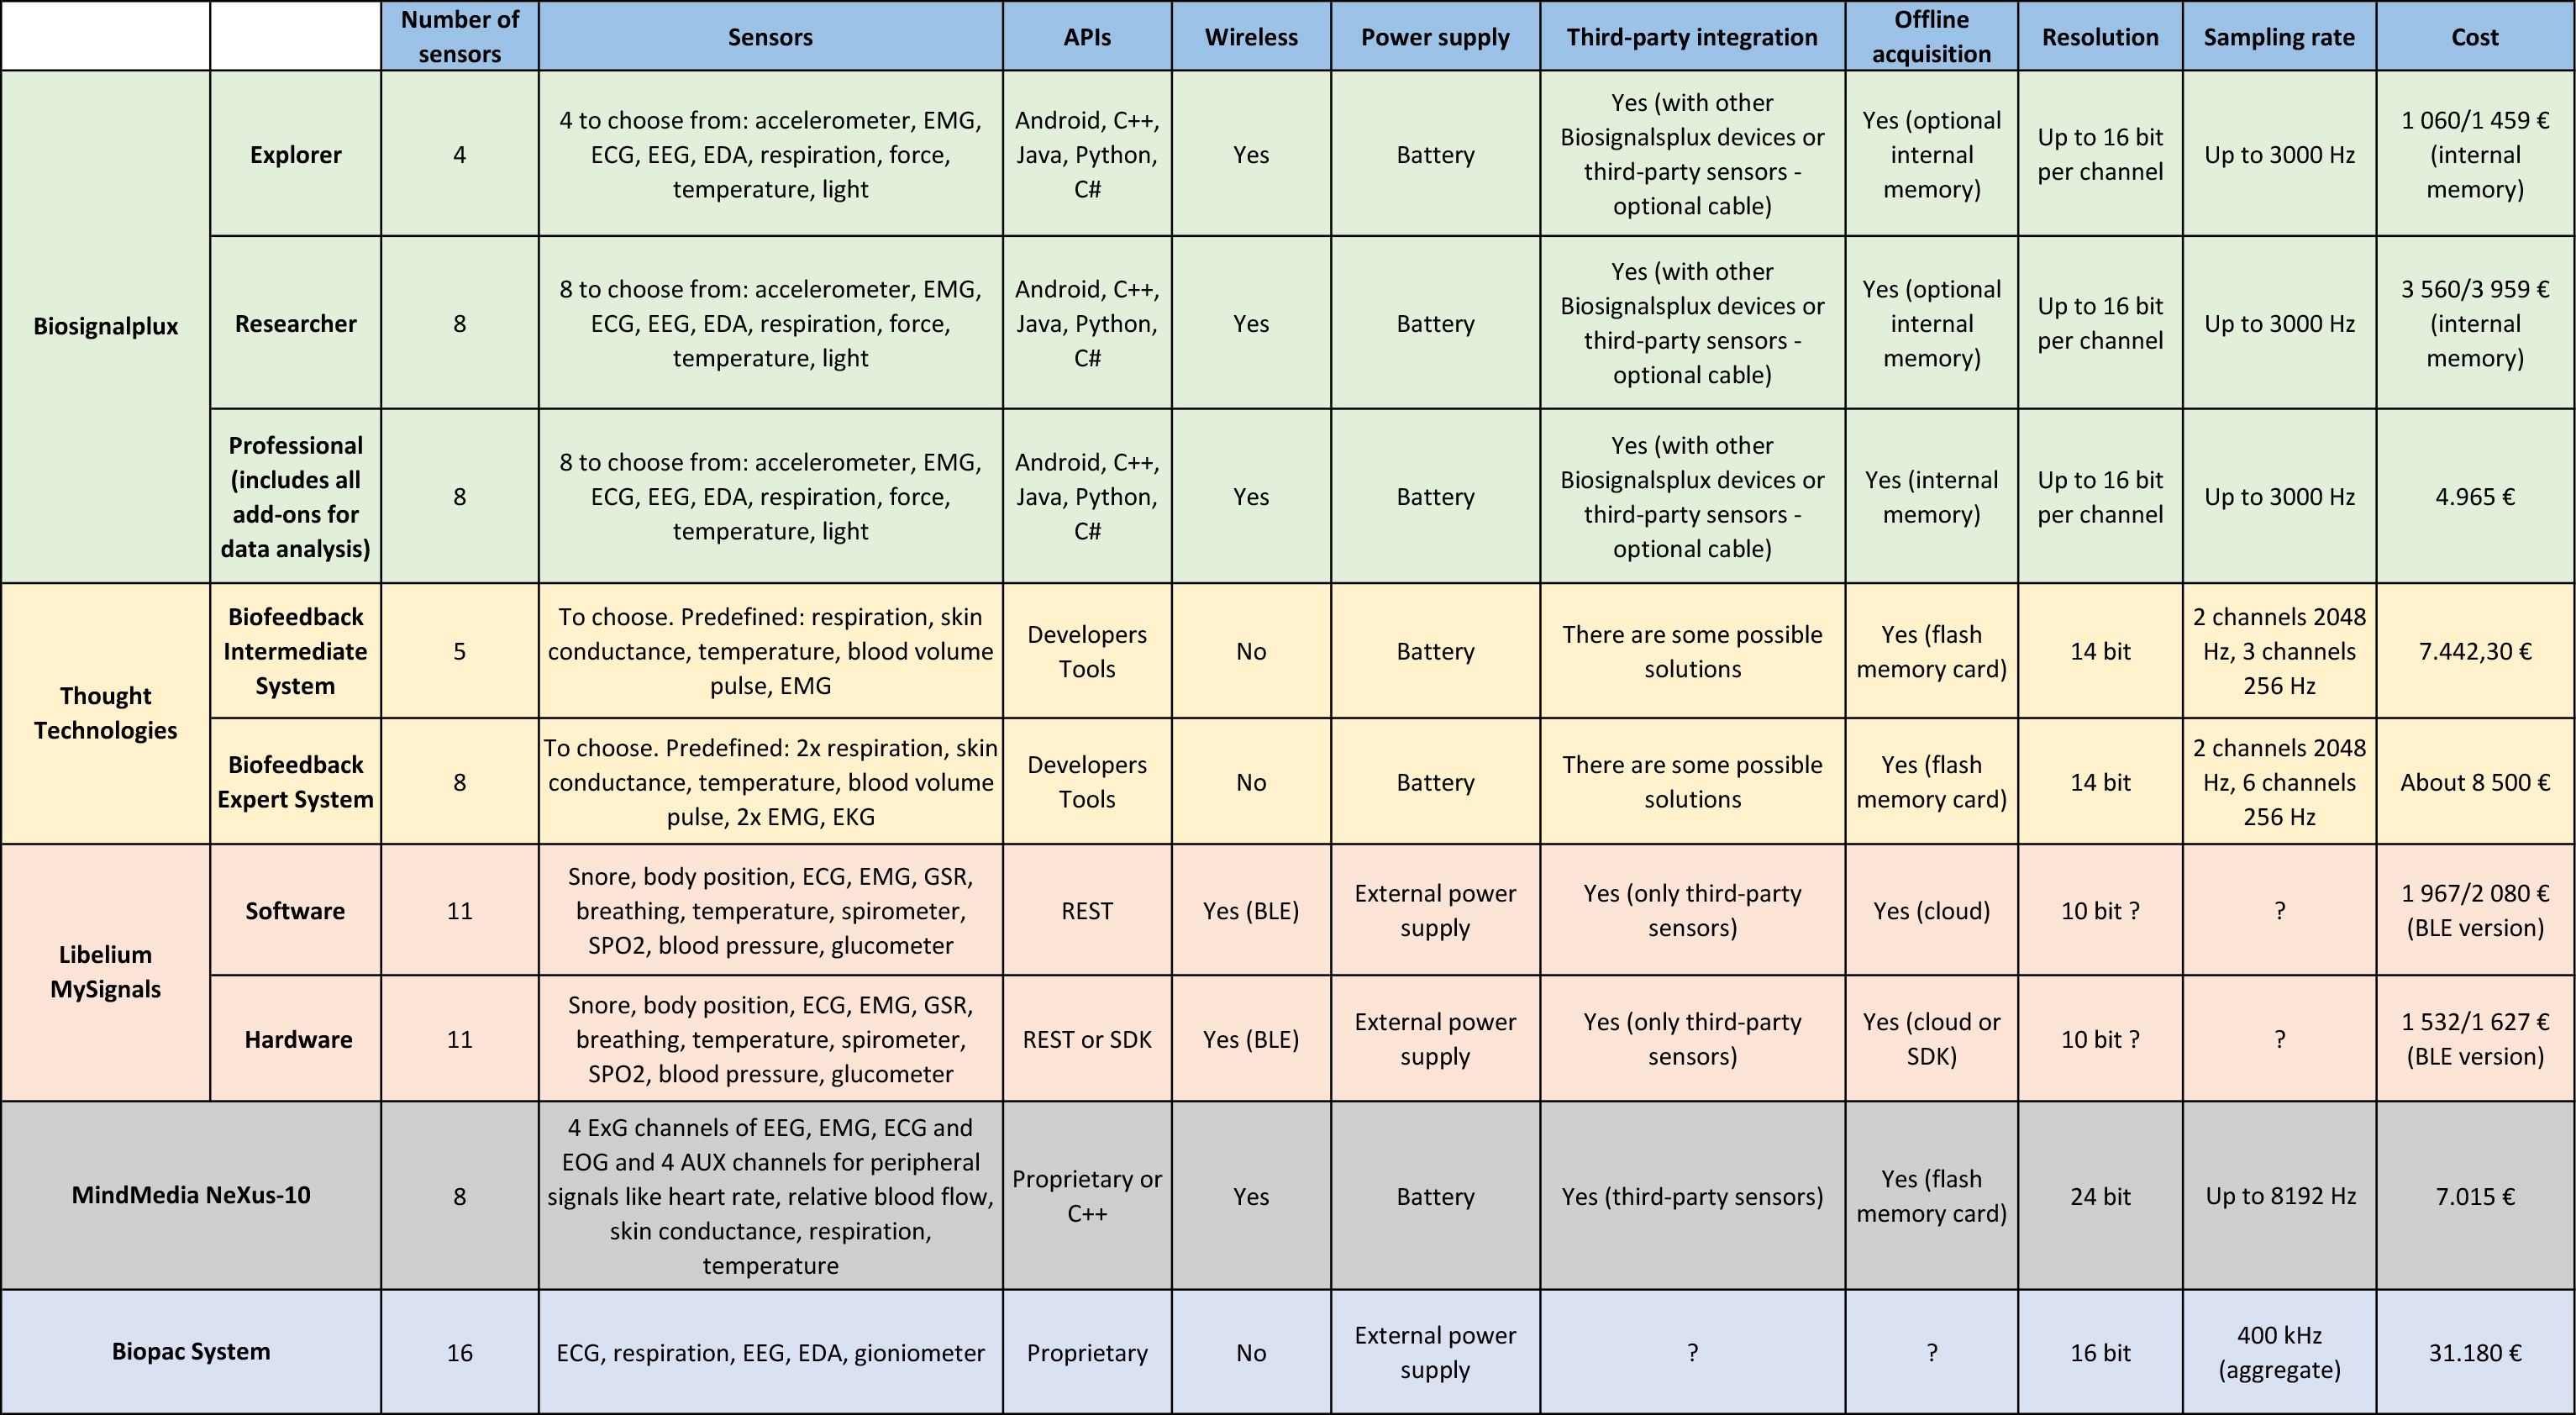
\includegraphics[scale=.9, angle=90]{images/table2}
\caption{Professional physiological kits comparison}
\end{figure}

\section{Used technologies}
This section presents the technologies used in the project and explains the reasons why they were chosen.

\subsubsection{Virtual reality}
The framework is meant to be used on a desktop environment, so for what concerns virtual reality the only possible choices were the Oculus Rift and the HTC Vive. The latter was the chosen one for the project. The main reason behind this decision was that it allows the user to physically move better than the Oculus, considering that its base stations can track a room-scale environment. Since the application can be used in a variety of different projects and experiments, this choice was the best for a general-purpose framework.

For what concerns the development environment of the virtual experience, the chosen tool was \textit{Unity3D}, a game engine available for Windows and MacOS that also supports virtual reality. Its scripting language is C\#, it is easy to use, compatible with HTC Vive and the created games can be launched in stand-alone mode, so it was the best choice for this project. 

\subsubsection{Programming language}
The application will handle the majority of the logic of the framework (see section \ref{sec:design}). It needs to be able to play videos easily and with the regular control commands (play, pause, stop), it has to support signals graphs representation and the development phase should not cost too much effort.
From these considerations we can conclude that the best programming language to use is Java. There are a lot of useful external libraries that can be imported from it, it has ready-to-use media player classes, nice graphical interfaces tools and it is cross-platform. 

\subsubsection{Physiological sensors}
The last choice to make is about which sensors to use in the framework.
There were several aspects that were taken into account in order to decide which professional kit was the best among those reported in figure 2.4. The kit should support the larger possible number of different sensors; it should be wireless, so that it is easier to connect and more practical to use; it should have internal memory and a battery, so that it can be also used for other kind of applications (e.g. external experiments); it should be compatible with third-party hardware or software and provide APIs in order to be usable with custom services and applications. The only option that satisfied all these condition was the BiosignalsPlux Researcher kit: 8 sensors, wireless, portable and with well documented API for several programming languages. The chosen sensors were: ECG, EMG, EEG, EDA, respiration, accelerometer (one channel per axis), temperature and force.


\chapter{Design}
This chapter describes the design of the system, starting from the initial idea and continuing with the multiple steps until the final scheme.

\section{Similar systems}
Before thinking about the design itself, a research on similar projects was conducted in order to better understand how this kind of systems are realized. The list includes not only projects that are close to this one as a whole, but also projects that provide just some similar features. Here follows the research result, divided in the various fields regarding the functionalities of the system. 

\begin{description}

\item [PhysioVR] \cite{munoz2016physiovr} is a framework developed to integrate physiological signals in mobile VR applications. Signals are acquired using wearable devices connected to the smartphone via Bluetooth and include heart rate, electroencephalography (EEG) and electromyography (EMG). The system allows to record data and to communicate with the VR content allowing an external event triggering using a real-time control.

\item [MuLES] \cite{cassani2015mules} is a tool for acquiring and streaming EEG signals that aims at facilitate the development of brain-computer interface programs. The system allows to replay a session and there are clients developed for use on different platforms and in various programming languages.

\item [PhysSigTK] \cite{rank2015physsigtk} is a toolkit for accessing low-cost physiological signals hardware from Unity. It aims at helping developers to exploit engagement in their effective games. 

\item [RehabNet] \cite{vourvopoulos2013rehabnet} is a system that helps patients rehabilitation through serious videogames that monitor physiological parameters. It supports a large variety of external physiological sensors. 

\item [Bicycle4CaRe] \cite{baldassini2017customization} is a tool for domestic physical training that uses VR and sensors to monitor user's activity. It simulates a home environment and collects data both from it and from the user, providing real-time feedback.

\item [Cube] \cite{cepisca2015platform} is a VR simulation platform for the supervision of personnel working in critical infrastructures. It collects physiological data during the virtual experience to identify the optimal physiological profile of personnel for using it in real scenarios.

\item [Athena] \cite{mcgregor2017integrating} is an analytics platform that acquires data from a combat simulator, combining this data with physiological signals of the player, and sends him body feedback.

\item [VAST] \cite{kuriakose2015understanding} is a virtual reality system for social communication that also collects physiological signals to determine the user's anxiety level.

\item [VR-SAAFE] \cite{bekele2017design} is a VR-based system developed for understanding facial emotions in subjects suffering of schizophrenia. The system uses an eye tracker and physiological signals to monitor user's eye gaze and emotions.

\end{description}

\subsection{Design}
The above systems use different approaches for what concerns design. 

\begin{itemize}

\item \textit{PhysioVR} is composed of two layers: the first one deals with synchronizing the devices and streaming the data, the second one is a Unity package that receives and analyzes data and physiological signals. There are also other two modules for external control and data recording.

\item \textit{MuLES} acts as the server part of a client-server architecture. It handles the communication between the several EEG sensors and transmits their data to the client applications. The devices are connected with their own drivers and the connection with the clients is realized through TCP/IP.

\item \textit{RehabNet} architecture is based on three building blocks: an hardware layer that deals with devices connection, a control panel that filters and cleans data, and a web interface for accessing the rehabilitation tools. The whole system is organized as a client-server application.

\item \textit{Bicycle4CaRe} is composed of different biofeedback devices connected to the PC via an Arduino board,ca desktop application and a VR simulated environment. The app contains the main functionalities and allows to control the experience.

\item \textit{Athena} is consists of a data acquisition layer that collects the signals from the sensors and the game data from the combat simulator. This layer sends data to IBM's Infosphere Streams, that processes it and generates analytics for storage.

\item \textit{VAST} is divided in three modules. The first one presents the tasks, the second one adapts and changes tasks according to the users behavior and the last one is the data acquisition layer. 

\item \textit{VR-SAAFE} is divided in three components too: task presentation environment based on Unity, eye tracking application and the physiological signals acquisition module.

\end{itemize}

\subsection{Physiological sensors}
This section presents the physiological sensors used by similar projects. This could help understanding which are the most used and useful signals in this kind of applications.
\textit{PhysioVR} uses only three signals: 

\begin{itemize}

\item heart rate, acquired through Android wearable devices such as smartbands, smartwatches or camera-based sensors;

\item EEG, obtained from a low-cost -wearable headband called Muse BCI;

\item EMG, acquired with Myo Armband, a device that contains 8 sensors and that recognizes gestures.

\end{itemize}
\textit{PhysSigTK} uses sensors considering criteria such as ease of use, price, software support and low-level access to data. Therefore the employed devices are four, measuring several different signals:  

\begin{itemize}

\item Empatica E3/E4, that measures EDA, blood volume, temperature and movement;

\item Wild Divine Iom, that provides skin conductance level (SCL) and heart rate;

\item e-Healt, an Arduino-based device that supports different sensors. In this case heart rate, galvanic skin response (a.k.a. EDA), ECG and breathing activity;  

\item NeuroSky Mindwave, a low-cost EEG sensor that also provides a heart rate sensor for the ear.

\end{itemize}
For what concerns \textit{RehabNet}, it uses protocols such as the \textit{Virtual-Reality Peripheral Network (VRPN)} and \textit{Open Sound Control (OSC)} for integrating a large variety of external devices and sensors (trackers, haptic devices, analog input, sound, etc). In addition to this, it natively supports three sensors:

\begin{itemize}

\item EEG acquired with Emotiv EPOC, a wireless EEG headset;

\item EMG, collected through Myomo mPower 1000, a prosthetic arm that also integrates sensors;

\item kinematic data, acquired with the Microsoft Kinect. 

\end{itemize}
\textit{VR-SAAFE} monitors physiological signals and eye gaze:

\begin{itemize}

\item Biopac Bionomadix measures PPG (from which heart rate can be extracted), skin temperature, EMG, respiration and galvanic skin response;

\item Tobii X120 for eye tracking. 

\end{itemize}
\textit{Bicycle4CaRe} measures both user's parameters and environmental conditions. The latter are not relevant for the project of this thesis; the former are:

\begin{itemize}

\item heart rate acquired with a pulse-oximeter sensor;

\item breath rate measured through a respiration monitor belt;

\item blood pressure collected with a sphygmomanometer. 

\end{itemize}

\subsection{Connectivity and libraries}
The project application will need to connect to the devices and to acquire signals. In order to be able to do it, similar systems techniques and methodologies were explored. Here are reported some examples of connectivity and external libraries approaches. 

\begin{itemize}

\item \textit{PhysioVR} transmits data over the UDP protocol. In this way the communication can be multicast and the transmission of all the physiological signals is done using a single port. Data can be accessed even from external devices with UDP capabilities. Users can access from remote and interact with the system bidirectionally, thus receiving data and sending feedback. The application also provides client scripts for different programming languages such as Java, C\#, Python, MATLAB.

\item \textit{MuLES} acquires data from the hardware using third-party APIs, SDKs, drivers or implementations of the specific device communication protocol. On the other hand, transmission to the client application is realized through the TCP/IP protocol, which allows to send data to a local network or over the Internet.
This means that client scripts can be written in any programming language supporting basic socket programming, such as Java or Python.

\item \textit{RehabNet} sends data to a smartphone running the app using a custom implementation of the UDP protocol. It also connects to an analysis and tracking tool. As anticipated above, the system makes use of VRPN and OSC protocols in order to connect to other external devices or libraries, for example the OpenViBE BCI software.

\item The interesting thing about \textit{Cube} is that it provides different connectivity solutions that can be used simultaneously or not. An example of it is ECG acquisition: it can be wired or wireless (Bluetooth) transmitted to a local machine, transmitted to a smartphone over the Internet or using a satellite connection

\end{itemize}

\subsection{Events and triggers}
Since the system should deal with key events and markers, here are presented the solutions adopted by \textit{PhysioVR} and \textit{Bicycle4Care}.

\begin{itemize}

\item \textit{PhysioVR} acquires data from the UDP connection and makes it available inside the Unity environment. This brings developers to have physiological data usable inside the experience, allowing some game parameters to be bound to physiological signals, or events to be triggered when certain conditions are verified. Another way of creating events is to have external inputs: the VR user can receive triggers influencing the experience scenario from an external application that monitors in real-time the person's vitals.

\item \textit{Bicycle4Care} reads data in real-time and guides the user through the experience with ad-hoc messages. Like for PhysioVR, events can be triggered when some parameter exceed a certain threshold. 

\end{itemize}

\subsection{Synchronization}
After the acquisition, data needs to be synchronized. Among the presented systems, only \textit{Athena} and \textit{VAST} use synchronization or explicitly write about it.

\begin{itemize}

\item \textit{Athena} acquires data from the combat simulator and the sensors and then it synchronizes them. This data is composed of physiological signals, game events like firing and target hits and haptic device activations. The adopted synchronization technique is not mentioned.

\item \textit{VAST} acquires real-time physiological signals and VR data in a synchronized manner for offline analysis. Markers are used to synchronize the different signals and the virtual environment. 

\end{itemize}

\subsection{Extensions}
This section is not related with similar systems but presents two ideas for extension and improvement of VR experiences that can be useful for the project development.

\begin{itemize}

\item The first idea comes from S. Otsuka and others, who think that physiological signals could be easier acquired if the sensors are embedded in a VR headset \cite{otsuka2017physiological}. They propose a new HMD that contains some sensors: their first prototype consists of a VR headset with an integrated PPG sensor that can measure heart rate. This system was tested and gave positive results, so this kind of devices could be a real and interesting thing for the future of VR and physiological signals research.

\item The second one is about VR and eye tracking. A paper about this is the one by Pradeep Raj and others \cite{kb2017gaze}. It presents the design of a VR-based social communication platform integrated with eye tracking technology. The authors believe that this kind of technology can be useful for presenting and analyze social situations and communication.

\end{itemize}

\section{Design}
\label{sec:design}
After analyzing similar systems with their potentially useful features, now we can introduce the actual design of this thesis project. 
Since there have been problems and changes during the development phase, the general design has been modified during the implementation of the system. 
The development was divided into three prototypes, each adding a new functionality to the system:

\begin{enumerate}
\item real-time visualization of the VR video, the camera video and the signals stream;
\item recording and synchronization of the streams;
\item replay of the streams and insertion of key markers.
\end{enumerate} 

Here are presented all the design prototypes, from the initial idea to the final result.

\subsection{Initial design}

\subsubsection{General architecture}

The system architecture follows the actors involved in the process: the user and the examiner. The participant is the person who takes part in the experiment: he is equipped with a VR headset (HTC Vive), physiological sensors (BiosignalsPlux kit) and a webcam pointing to his face. The communication between these sensors and the examiner's computer is realized through controllers. The examiner component is constituted by the controllers, a recording and synchronization layer that saves the data on the storage and a Java application used to see in real-time what the user is experiencing and to start/stop the recording. 
Concerning the offline mode of the system, it is represented by two additional blocks. The first one deals with the offline part of the application itself, while the other represents the external applications that can be used to analyze data (e.g. MATLAB or Python). This last part is not covered by the project.
Figure 4.1 shows an overall view of the system.

\subsubsection{Controllers}

Regarding the controllers, in the initial design they communicate with the Java application, that executes every task.
In this case the application represents both the real-time and offline Java applications showed in figure 4.1.
Starting from VR, the development platform is Unity and to send the video stream to the Java application we are going to use the \textit{RockVR} plugin, which allows to record a video of what the user sees through the headset and send it to a streaming server in real time. The application is then going to read the stream and play it using the \textit{MediaPlayer} Java class. For the physiological sensors we can use the official \textit{Plux} API, which allows to easily acquire the signals data from Java.
Finally, for the webcam we are going to use the \textit{JavaCV} library, a wrapper of the \textit{OpenCV library}, for visualizing and recording the video stream. For a detailed description of these tools and libraries see section \ref{sec:thirdparty}. The controllers schema is represented in figure 4.2.

\begin{figure}
\centering
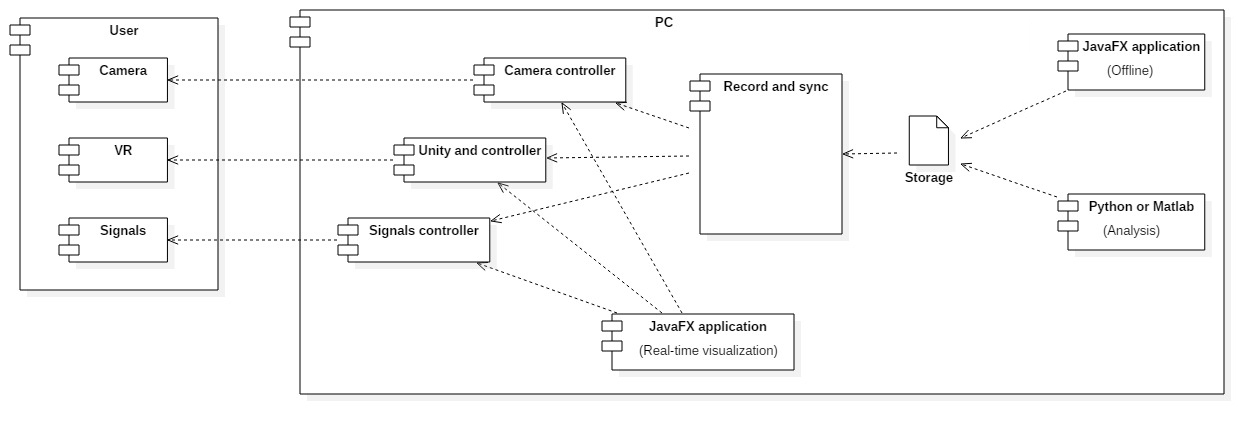
\includegraphics[scale=.5, angle=90]{images/general_schema}
\caption{Initial general architecture}
\end{figure}

\begin{figure}
\centering
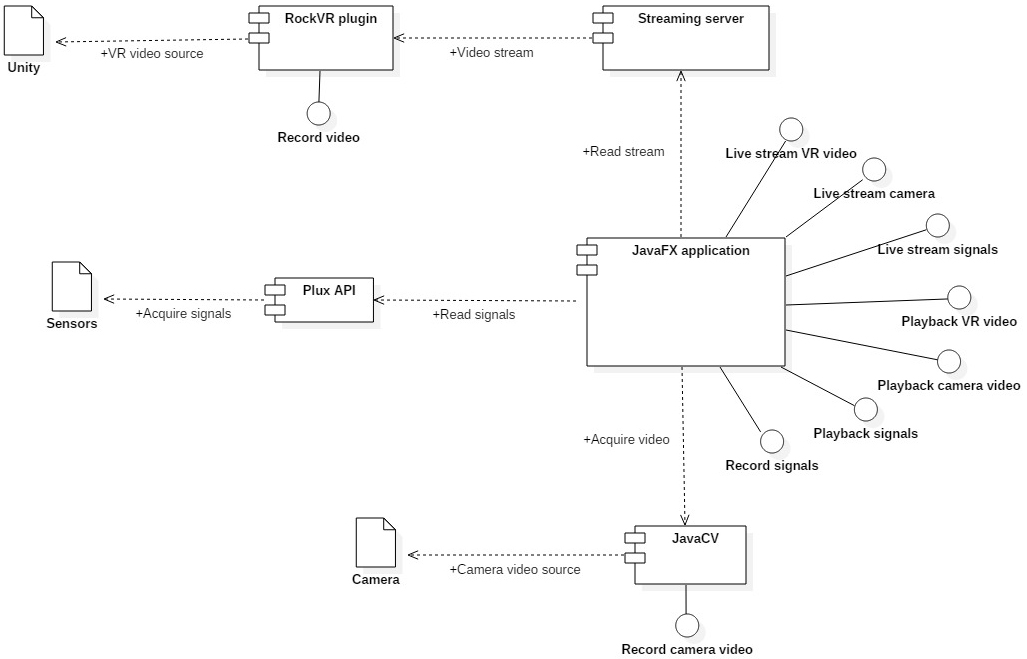
\includegraphics[scale=.57, angle=90]{images/2_controllers2}
\caption{Controllers initial schema}
\end{figure}

\subsection{First prototype}

\subsubsection{Original schema}
The first prototype only concerns the real-time visualization of the VR video, the camera video and the signals stream. Therefore, we can focus on the left side of figure 4.1: we only consider the user, the controllers and the real-time visualization application (figure 4.3). For what concerns the controllers, we are interest only in the real-time tasks, so the diagram is the one in figure 4.4.

\begin{figure}
\centering
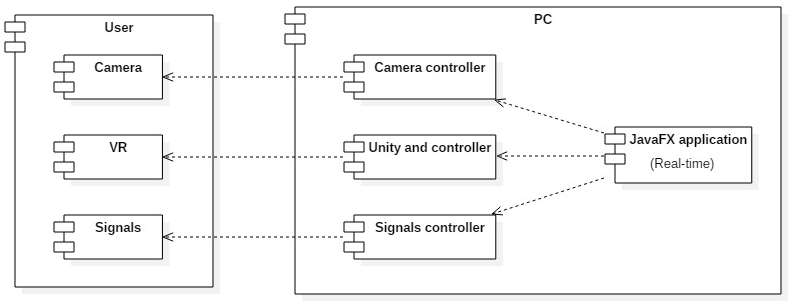
\includegraphics[scale=.5]{images/prot1_initial_design}
\caption{First prototype original architecture}
\end{figure}

\begin{figure}
\centering
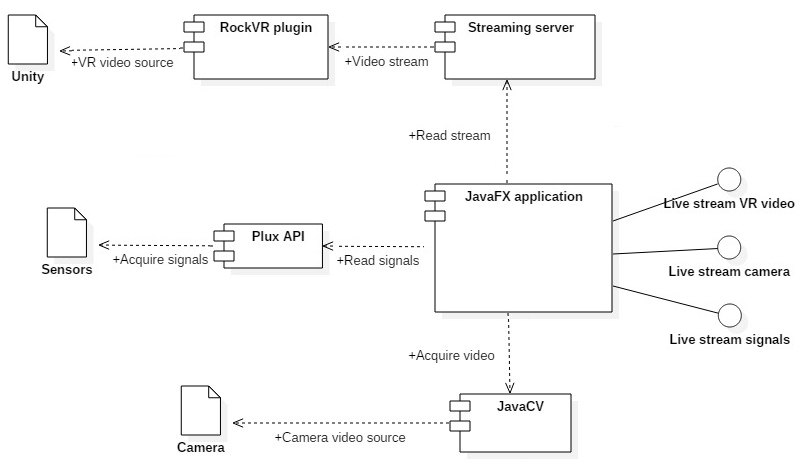
\includegraphics[scale=.5]{images/prot1_controllers_original2}
\caption{First prototype controllers original schema}
\end{figure}

\subsubsection{Implementation changes}
The original diagrams changed when implementing the prototype. The main problem was about the VR video streaming: encoding it, sending it to the streaming server (localhost) and decoding it generated a delay of about 3 seconds. This resulted in an out of sync visualization, since camera and physiological signals were synchronized but VR was not. This behavior was not acceptable. Even if it could have been possible to synchronize the three sources after the recording, it was not possible to see everything in real-time, failing to satisfy the first requirement.

Trying to find a solution to this problem was not easy. Playing the VR video stream from the Java application means to export what happens in Unity and to read it from an external application. The only suitable technique found was the above one. With it not working, the only reasonable solution was to use two screens and split the real-time part of the application in two pieces: one handling camera and signals visualization and one the VR visualization. The former will be handled by the Java application itself on the first screen and the latter by Unity on the second screen (figure 4.5).

\begin{figure}[h]
\centering
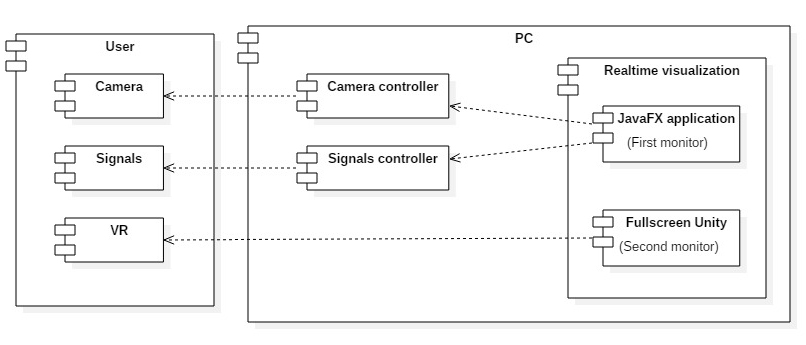
\includegraphics[scale=.5]{images/prot1_implementation}
\caption{First prototype architecture implementation}
\end{figure}

As regards the controllers, we can simply get rid of the VR part because it has no more connections with the main application (figure 4.6).

\begin{figure}[h]
\centering
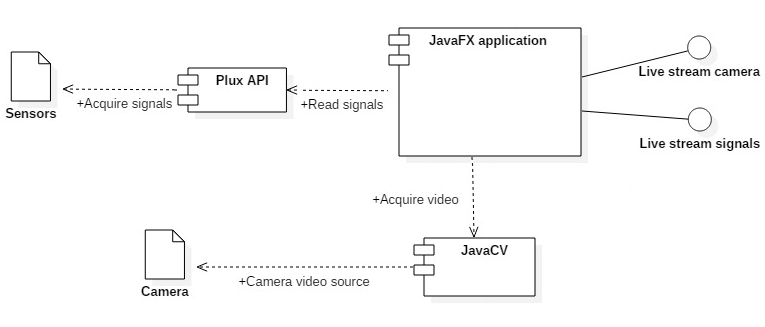
\includegraphics[scale=.51]{images/prot1_controllers_implementation2}
\caption{First prototype controllers implementation}
\end{figure}

\subsection{Second prototype}
The second prototype was supposed to add the recording functionality to the system. The general schema is exactly the same as the one in figure 4.5, but with the addition of the \textit{Record and sync} module and of the storage (figure 4.7). 

\begin{figure}[h]
\centering
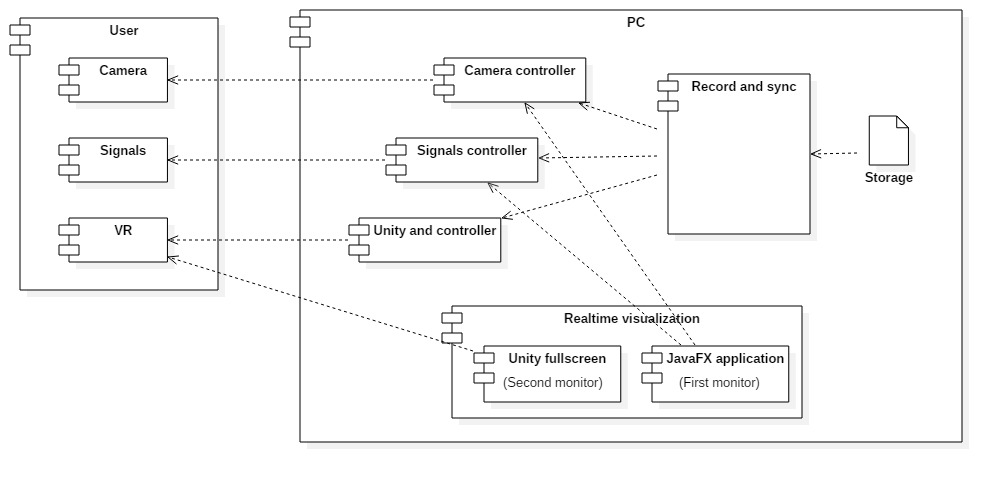
\includegraphics[scale=.41]{images/prot2_general}
\caption{Second prototype architecture}
\end{figure}

Since from the first prototype architecture change we can not visualize the VR video in real-time from the Java application, we can not record it either, so we need to do it from Unity itself. This is the reason why there is also a Unity controller in the diagram (figure 4.8): this component is the RockVR plugin, and it will handle the recording of what the user sees and store it on the hard drive. 

\begin{figure}[h]
\centering
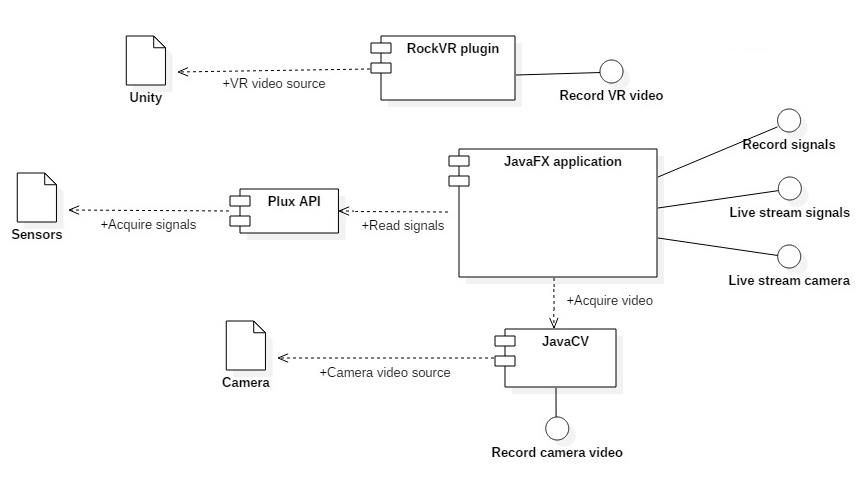
\includegraphics[scale=.47]{images/prot2_controllers2}
\caption{Second prototype controllers}
\end{figure}

This new consideration brings the system to be composed of two modules: the first one is a Java application that plays and records the camera and signals streams, the second one is a Unity package that records the VR video.
At the end of the acquisition, the 3 files – VR video, camera video and signals data – are synchronized (see section \ref{sec:sync}) in order to be replayed and analyzed properly.

\subsection{Third prototype}
The third and last prototype represents the final version of the system. It adds the replay feature to the application, included the option to insert markers on specific moments of the playback. 

Both the architecture and the controllers schemas are similar to the initial idea one, except for the separation of Java and Unity blocks (figure 4.9 and 4.10). 

\begin{figure}[h]
\centering
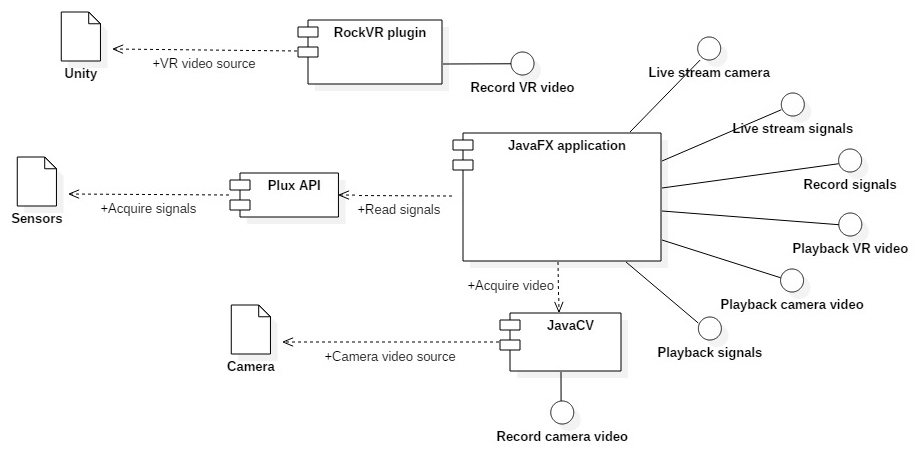
\includegraphics[scale=.44]{images/prot3_controllers2}
\caption{Third prototype controllers}
\end{figure}

\section{Synchronization}
\label{sec:sync}
Synchronization can be considered as one of the most important parts of this project. The value of the framework is that it gives researchers the possibility to have a ready-to-use environment that allows them to save valuable time, since everything they record can be easily synchronized.
This section gives an overview of the synchronization problem and describes the solution adopted to solve it.

\begin{figure}[p]
\centering
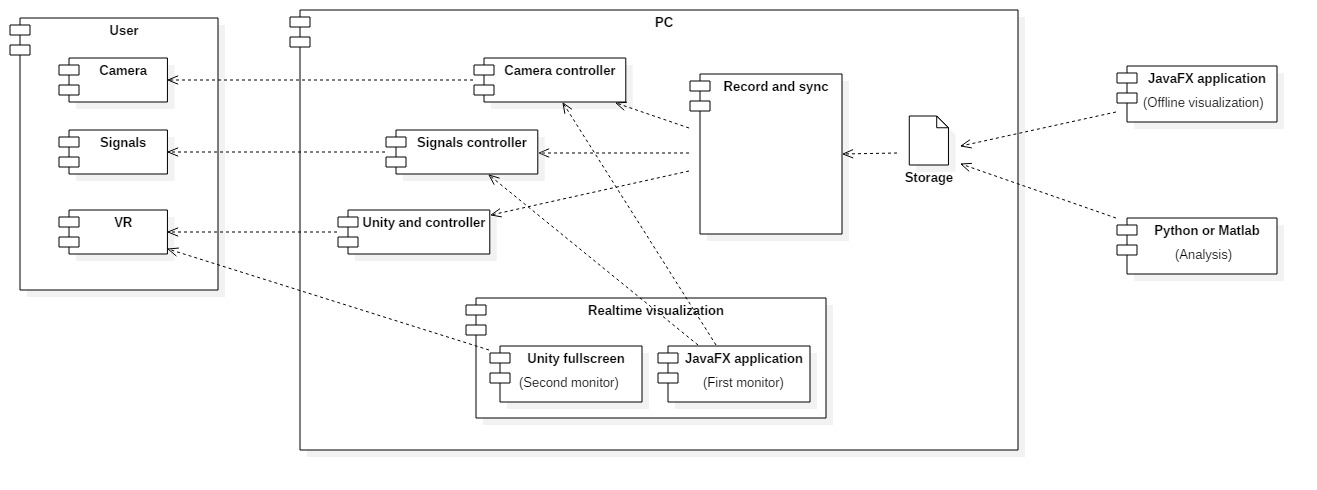
\includegraphics[scale=.5, angle=90]{images/prot3_architecture}
\caption{Third prototype architecture}
\end{figure}

\subsubsection{Synchronization issue}

The camera video and the signals are acquired from the same application. Since the recording starts when the examiner clicks a button, both the sources start being stored approximately at the same time. There should be no relevant delays (i.e. more than one or two tenths of a second), therefore they should be already synchronized. This means that if the implementation is done correctly, the camera video and the signals file do not need further processing in order to be synchronized.

The problem arises when we also consider VR video. As stated above, it is displayed on the Unity window itself and is recorded through a plugin. Just as the other recording, also this one is initiated by the examiner: since the two recordings events are generated by a human actor, there is no way they start at the exact same time. 

We can consider the following as an example of a real usage of the platform. The examiner has already run the application and Unity, configured everything and started seeing the streams in real-time. Now he wants to record the whole session. He first starts recording from the Java application, acquiring signals and camera video, and then switches to the second screen and starts recording from Unity. Even if this two actions are executed very quickly, there will be an unavoidable delay (at least half a second) between the two recordings.
This fact is not acceptable with respect to the framework idea and requirements, thus we need to find a way to really synchronize the files. 
Synchronization means to align the files or to cut them in order to display at the same moment events and data that happened at the same time. The ideal solution would have been to find a way of starting the two recordings simultaneously, without the double intervention of the examiner. This would have required some kind of connection between Java and Unity and was not easy to achieve. The solution adopted to address the problem was another: employ system timestamps.

\subsubsection{System timestamps}

Timestamps are sequences of characters representing a time unit, generally indicating a date and a time. In this case the used timestamps are the \textit{Unix timestamps}, referring to the total number of seconds elapsed since midnight, January 1, 1970 UTC. When retrieved from a computer, this value depends on the underlying operating system. OS in fact measure time with different milliseconds granularity, for example Windows used 55 milliseconds until the 98 version and 10 milliseconds after. 

The general idea about how to use timestamps for synchronization is to associate to each recorded file the timestamp, in milliseconds, of the moment when the recording starts. This gives us the indication about the time when the recordings started and therefore we can compute the difference between the values to get the exact delay between a source an another. The same steps are applied to the end of the recordings. 

An overview on the synchronization phase can be described as follows. Without loss of generality we can assume that the examiner starts (and stops) recording from the Java application and then continues with Unity:

\begin{enumerate}

\item examiner starts the recording from the Java application;

\item current timestamp is associated to signals and camera video files as \textit{initial timestamp};

\item signals and camera video streams begin to be saved on the storage;

\item examiner starts the recording from Unity;

\item current timestamp is associated to VR video file as \textit{initial timestamp};

\item VR video stream begins to be saved on the storage;

\item examiner stops the recording from the Java application;

\item current timestamp is associated to signals and camera video files as \textit{final timestamp};

\item signals and camera video streams stop to be saved on the storage;

\item examiner stops the recording from Unity;

\item current timestamp is associated to VR video file as \textit{final timestamp};

\item VR video stream stops to be saved on the storage;

\item difference between signals (same as camera) and VR initial timestamps is computed (we can name this value ); 

\item difference between signals (same as camera) and VR final timestamps is computed (we can name this value \textit{delayEnd}); 

\item first \textit{delayStart} milliseconds of signals and camera video files are cut;

\item last \textit{delayEnd} milliseconds of VR video files are cut.

\end{enumerate}

This procedure guarantees a good level of synchronization, which basically relies on timestamps accuracy. All the information about source files and timestamps is stored on simple text files. Implementation details about synchronization are reported in section \ref{sec:syncrealization}.


\chapter{Realization}
After the complete design of the system, it is time to talk about the actual implementation. This chapter explains some realization choices and gives details about core parts of the application.

\section{Main development phases}
Despite Java is a cross-platform language, Unity is only available for Windows and MacOS, and the former is more widespread that the latter. That is why the chosen operating system for the development and deployment of the framework was Windows. 
The development tool for the application was \textit{NetBeans}, an integrated development environment (IDE) originally released for Java, but then expanded to support also other programming languages such as C, C++ and Javascript.
Since the application needs to make use of external libraries, the best option was to use the build automation tool \textit{Apache Maven}.
It allows to easily describe dependencies and integrate libraries and plugins in the project, downloading them from repositories. 

\subsection{GUI}
For what concerns the graphical interface of the application, the selected tool was \textit{JavaFX}, a software platform for creating desktop applications. It aims at being the replacement of Swing as the standard GUI library for Java applications. Latest versions of JavaFX use \textit{FXML}, an XML-based markup language, for defining user interfaces. The platform also provides a scene builder to create scenes by dragging and dropping components into it; this information is saved as FXML code, whose variables can be referred from Java controllers using the annotation \textit{@FXML}. 

The graphical interface structure is very basic and simple, providing only the really necessary components. The application is divided in two parts named  and \textit{Offline mode}, each with its own user interface. Their layouts are very similar, the only big difference is that the former contains signals configuration controls while the latter also includes VR video playback.
The general idea is to have the screen horizontally split in half. The bottom part shows the signals while the upper part is in turn divided in two slices, one for the camera and one for the signals configuration (or VR video playback). Figure 4.1 shows an empty \textit{Real-time mode} GUI. 

\begin{figure}[p]
\centering
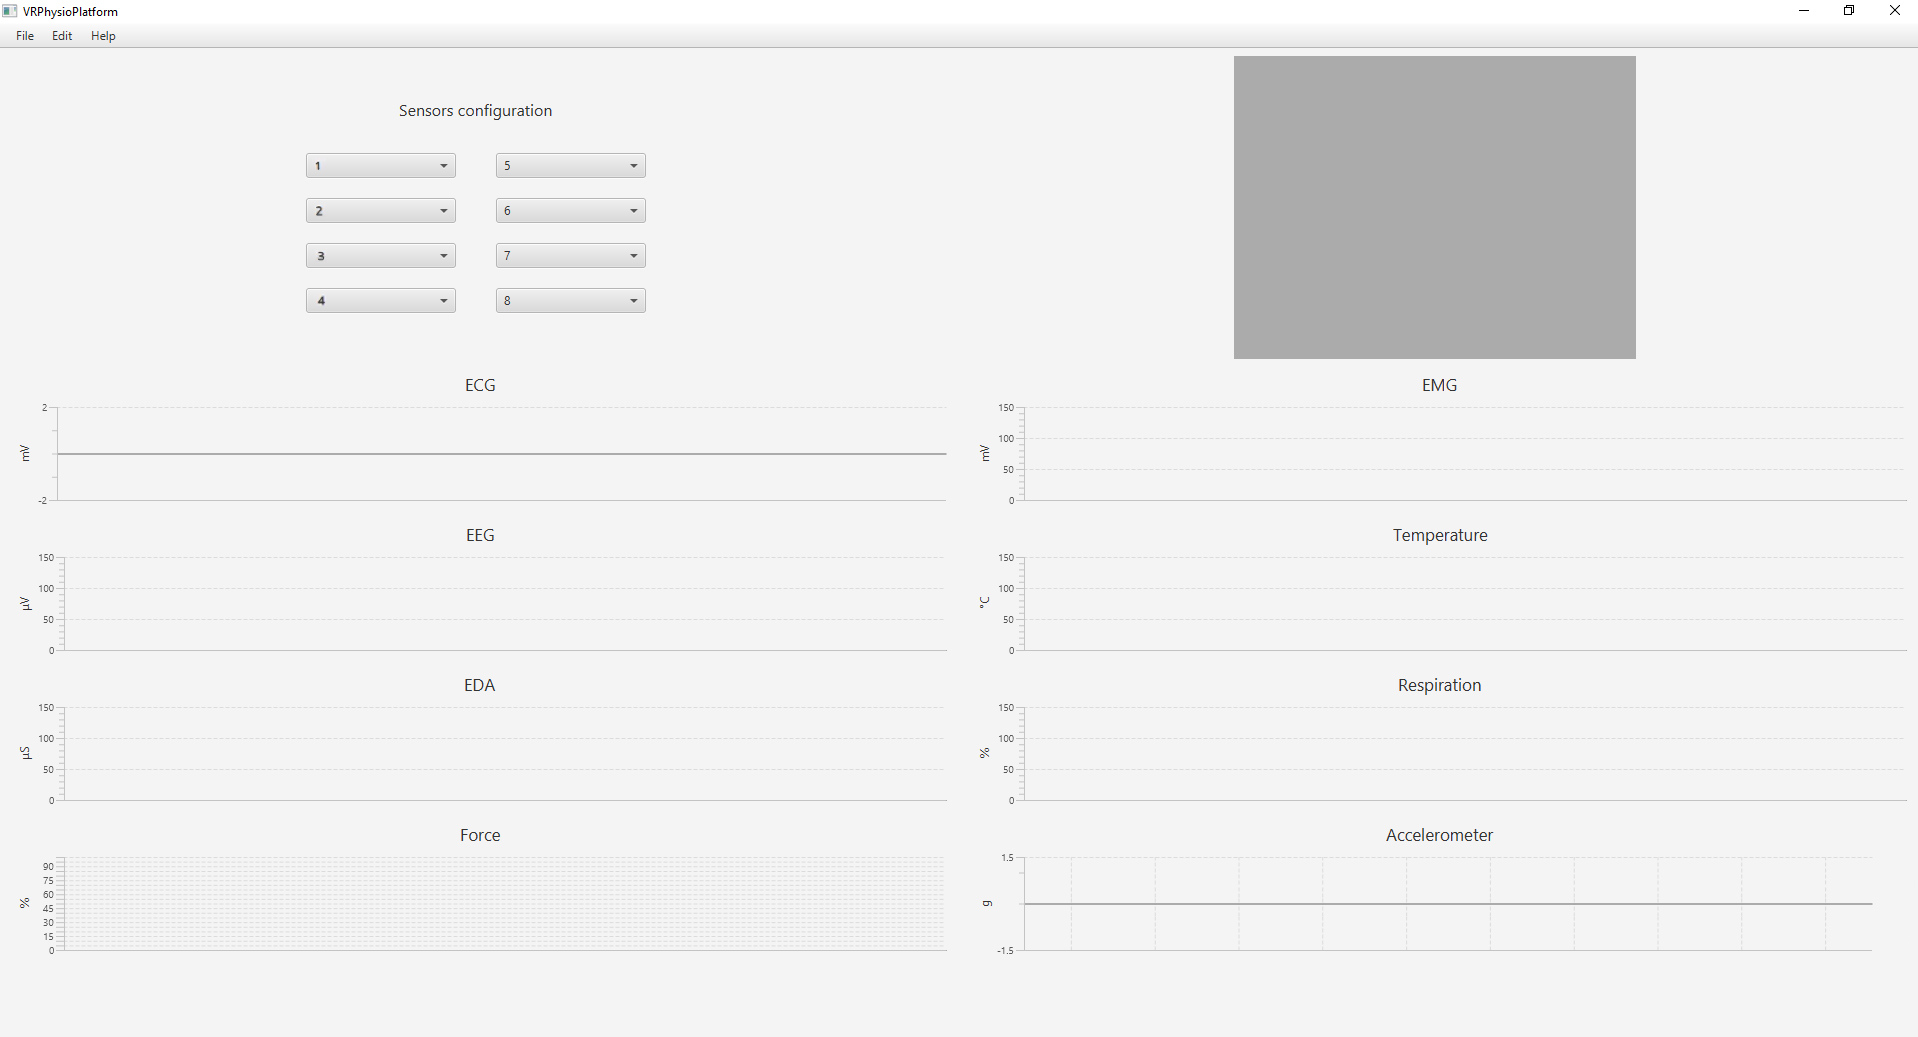
\includegraphics[scale=.46, angle=90]{images/realtime2}
\caption{Real-time mode user interface}
\end{figure}


\subsection{First prototype}
The first prototype just had to show signals data and camera and VR videos in real-time. As already explained in the \textit{Design} chapter, the real-time part pf the framework is divided in two pieces, one is the Java application, handling signals and camera video, and the other is Unity, showing the VR video. For what concerns Unity we do not need any development for this prototype, considering that we are only interested in seeing what the participant sees and Unity already does it in its predefined settings. When the virtual scene starts, it can be played in full-screen mode so that it is easy for the examiner to follow the participant's movements.

Regarding the other application, in this phase it has to be able to display camera video and physiological signals in real-time. Let us start with the camera. 

\subsubsection{Camera}

The camera used during the whole development and testing of the system was a \textit{Logitech} HD webcam connected to the computer via USB. As anticipated above, the software controller that makes camera accessible from Java is the \textit{JavaCV} library (see section \ref{sec:thirdparty}). It provides several methods for capturing and recording camera frames. 

Going into implementation details of this feature, \textit{OpenCVFrameGrabber} class is used to deal with camera input frames. First we need to create a new instance of the class passing as an argument the code of the camera. If the HTC Vive is also connected to the computer we have two active cameras, so the best thing to do is to give 0 as a parameter: this will make the system use the default camera or show a dialog to the user, who can select the one he wants. Next step is to call the \textit{start()} method on the created instance. This causes the object to grab frames from the camera until the \textit{stop()} command is called. In order to handle the incoming stream without blocking the whole execution we need to dedicate a new thread to it. This thread will execute a \textit{Runnable} that captures and displays a frame placing it into an \textit{ImageView}. First the grabber grabs a frame, then this frame is converted into an image that can be set into the ImageView.

When dealing with a graphical interface, every update of it should be executed on the JavaFX Application Thread. To solve this issue, the \textit{setImage(image)} method was called inside a runnable passed as an argument to \textit{Platform.runLater(Runnable runnable)}. This method makes sure that the specified runnable gets executed on the main thread at some unspecified time in the future.

In order to obtain a video containing 30 frames per second (FPS), the grabbing code was executed once every 33 milliseconds. This result was achieved thanks to the usage of the \textit{ScheduledExecutorService} class. Code snippet 4.1 shows in details the described procedure.
\\
\renewcommand{\lstlistingname}{Code snippet}
\begin{lstlisting}[caption={Camera input management}, captionpos=b]
import java.util.concurrent.Executors;
import java.util.concurrent.ScheduledExecutorService;
import java.util.concurrent.ScheduledThreadPoolExecutor;
import java.util.concurrent.TimeUnit;
import org.bytedeco.javacv.Frame;
import org.bytedeco.javacv.FrameRecorder;
import org.bytedeco.javacv.FrameGrabber;
import org.bytedeco.javacv.FFmpegFrameRecorder;
import org.bytedeco.javacv.Java2DFrameConverter;
import org.bytedeco.javacv.OpenCVFrameGrabber;
...
private ScheduledExecutorService cameraTimer;
private OpenCVFrameGrabber grabber;
private Java2DFrameConverter converter;
@FXML
private ImageView cameraView;
...

grabber = new OpenCVFrameGrabber(0);
converter = new Java2DFrameConverter();

try {
	grabber.start();
} catch (FrameGrabber.Exception ex) {
	logger.log(Level.SEVERE, "Error while initiating frame grabber", ex);
}

cameraTimer = Executors.newSingleThreadScheduledExecutor();
cameraTimer.scheduleAtFixedRate(new CameraRunnable(), 0, 33, TimeUnit.MILLISECONDS);

...
        
class CameraRunnable implements Runnable {

    @Override
    public void run() {
        Frame capturedFrame = null;
        try {
            capturedFrame = grabber.grab();
        } catch (FrameGrabber.Exception ex) {
            logger.log(Level.SEVERE, "Error while grabbing frame", ex);
        }

        Image image = SwingFXUtils.toFXImage (converter.convert(capturedFrame), null);  
            
        Platform.runLater(new Runnable() {
            @Override
            public void run() {
                cameraView.setImage(image);
            }
        });        
    }
}
        
\end{lstlisting}

\subsubsection{Physiological signals}
The other feature we need to implement for this prototype is signals data visualization. BiosignalsPlux device is connected to the computer wireless, using an included Bluetooth dongle.
The communication between the device and Java is realized through the official Plux Java API (see section \ref{sec:thirdparty}). This consists of a collection of basic classes and methods useful for retrieving sensors signals. The main class is \textit{Device}, which represents the Plux device; the \textit{Frame} class models a frame of acquired data and consists of a sequence number (byte), a boolean indicating the state of the digital input and the actual data. This is represented as an array with 8 elements (16 bits each), one per channel. Before starting the acquisition we need to find the connected device with the \textit{Device.FindDevices(Vector v)}, which stores in \textit{v} the MAC addresses of the discovered devices. Once found, a new Device object is created and the acquisition is started. Just as camera stream, also for signals we need a new thread to acquire data without freezing the whole application. Since Plux device reads data with a sampling rate of 1 kHz, (i.e. 1000 data frames per second), the thread is scheduled to be executed once every millisecond and it simply gets one single frame, storing it in a \textit{Frame} object.
\\
\begin{lstlisting}[caption={Sensors data acquisition}, captionpos=b]
import java.util.Vector;
import plux.newdriver.bioplux.*;
...
private String deviceMAC;
private Device dev;
private Device.Frame[] frames;
private ScheduledExecutorService signalsTimer;
...
Vector devs = new Vector();
        
try {
	Device.FindDevices(devs);          
            
	if (devs.isEmpty()){
		Alert alert = new Alert(AlertType.ERROR, "Impossible to connect to the sensors. Please verify the connection and try again.");
		alert.setTitle("Sensors not found");
		alert.showAndWait();
    }
    else {
    	deviceMAC = (String) devs.get(0);
		dev = new Device(deviceMAC);
		frames = new Device.Frame[1];
		frames[0] = new Device.Frame();
		dev.BeginAcq(1000, 0xFF, 16); // 1 kHz, 8 channels, 16 bits
    }
}
catch (BPException err){
	logger.log(Level.SEVERE, "Error while initializing the device", err); 
}   

if (!devs.isEmpty()){
	...
	Thread getSignals = new Thread(() -> {
		try {
    		dev.GetFrames(1, frames);
    		...
    	} catch (BPException ex) {
    		logger.log(Level.SEVERE, "Error while getting the frames", ex);
    	}
	});

	signalsTimer = Executors.newSingleThreadScheduledExecutor();
	signalsTimer.scheduleAtFixedRate(getSignals, 0, 1, TimeUnit.MILLISECONDS);
}
        
\end{lstlisting}

Once acquired, signals data need to be visualized. JavaFX provides chart components that can be used to plot the data. For this kind of signals the best plot type is the line chart; we assign a chart to each signal source. The corresponding Java class is \textit{LineChart<X,Y>}, where X and Y are the axis to be used. In this case we use a number containing the time value as X and a number indicating the sensor signal as Y. The easiest way of populating a chart is to add a \textit{XYChart.Series<X,Y>} to it. This class is used to insert actual data to the chart. A series is assigned to the corresponding chart only when the examiner sets it in the \textit{Sensors configuration} panel; the reason behind this behavior is explained in section \ref{subsec:secondprot}. Once added to the chart, the series need to be regularly updated so that they can show the signals stream. The class that is commonly used in this kind of scenarios is \textit{Timeline}, that allows to define an animation for a JavaFX object. The sensors provide 1000 frames per second but they are too many for visualization, so we can choose to only read some values. A good trade-off is to display 10 frames per second, i.e. to update the chart every 100 milliseconds: this is the value we set for the animation. Every time the animation is executed, the current data frame is read and the series is updated, therefore updating also the chart. 

\begin{figure}[h]
\centering
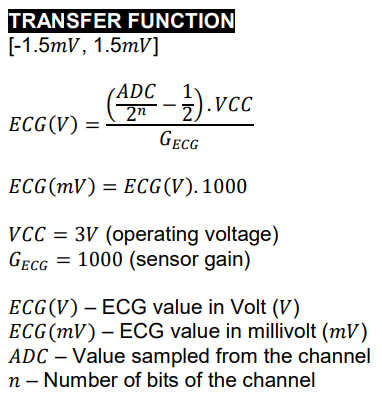
\includegraphics[scale=.4]{images/transfer_function}
\caption{ECG sensor transfer function}
\end{figure}

Sensors acquire data with a 16 bits resolution, meaning that raw data consists of values ranging from 0 to 65335. To transform this numbers into meaningful measure values we need transfer functions. BiosignalsPlux provides datasheets containing information for each sensor including transfer functions. For example for the ECG sensor the function transforms the raw data into a value ranging from -1.5 mV to 1.5 mV. Figure 4.2 shows the ECG sensor transfer function.
Functions were easily implemented in Java and used to plot the signals charts. 
Code snippet 4.3 shows the main parts of this phase, taking as an example the ECG chart; every other chart is visualized with the exact same code. 
\\
\begin{lstlisting}[caption={Sensors data visualization}, captionpos=b]
import javafx.scene.chart.LineChart;
import javafx.scene.chart.XYChart;
import javafx.animation.KeyFrame;
import javafx.animation.Timeline;
...
@FXML
private LineChart<Number, Number> ecgChart;
private XYChart.Series<Number, Number> seriesEcg;
...
seriesEcg = new XYChart.Series<>();
seriesEcg.setName("ECG");
for (int i = 0; i < 10; i++)
	seriesEcg.getData().add(new XYChart.Data<>(i, 0));

comboBox1.valueProperty().addListener(new ChangeListener<String>() {
	@Override
    public void changed(ObservableValue<? extends String> observable, String oldValue, String newValue) {
    	...
    	if (newValue != null){
        	switch (newValue){
        		...
        		case "ECG":
                	if (!ecgChart.getData().contains(seriesEcg)){
                    	ecgChart.getData().add(seriesEcg);
                    	...
                    }
                ...
            }
        }
    }
});

Timeline updateGraphs = new Timeline(new KeyFrame(Duration.millis(100), (ActionEvent event) -> {
	try {
		if (seriesEcg.getData().size() >= 10){
			seriesEcg.getData().remove(0);
			...
		}
		
		Device.Frame data = frames[0];
		
		seriesEcg.getData().add(new XYChart.Data<>(signalsCounter, transEcg(data.an_in[ecgPos]))); //transfer function
		...
		signalsCounter++;

	} catch (Exception ex) {
		logger.log(Level.SEVERE, "Error while updating charts", ex);
	}
}));
updateGraphs.setCycleCount(Timeline.INDEFINITE);
updateGraphs.play();

\end{lstlisting}

%Unity???

After the above steps the first prototype was ready and able to read physiological signals and camera video. On the other side, Unity could make the examiner follow the participant's visual experience. Figures 4.3 and 4.4 show what Prototype 1 looks like. An example scene was used for Unity.

\begin{figure}[p]
\centering
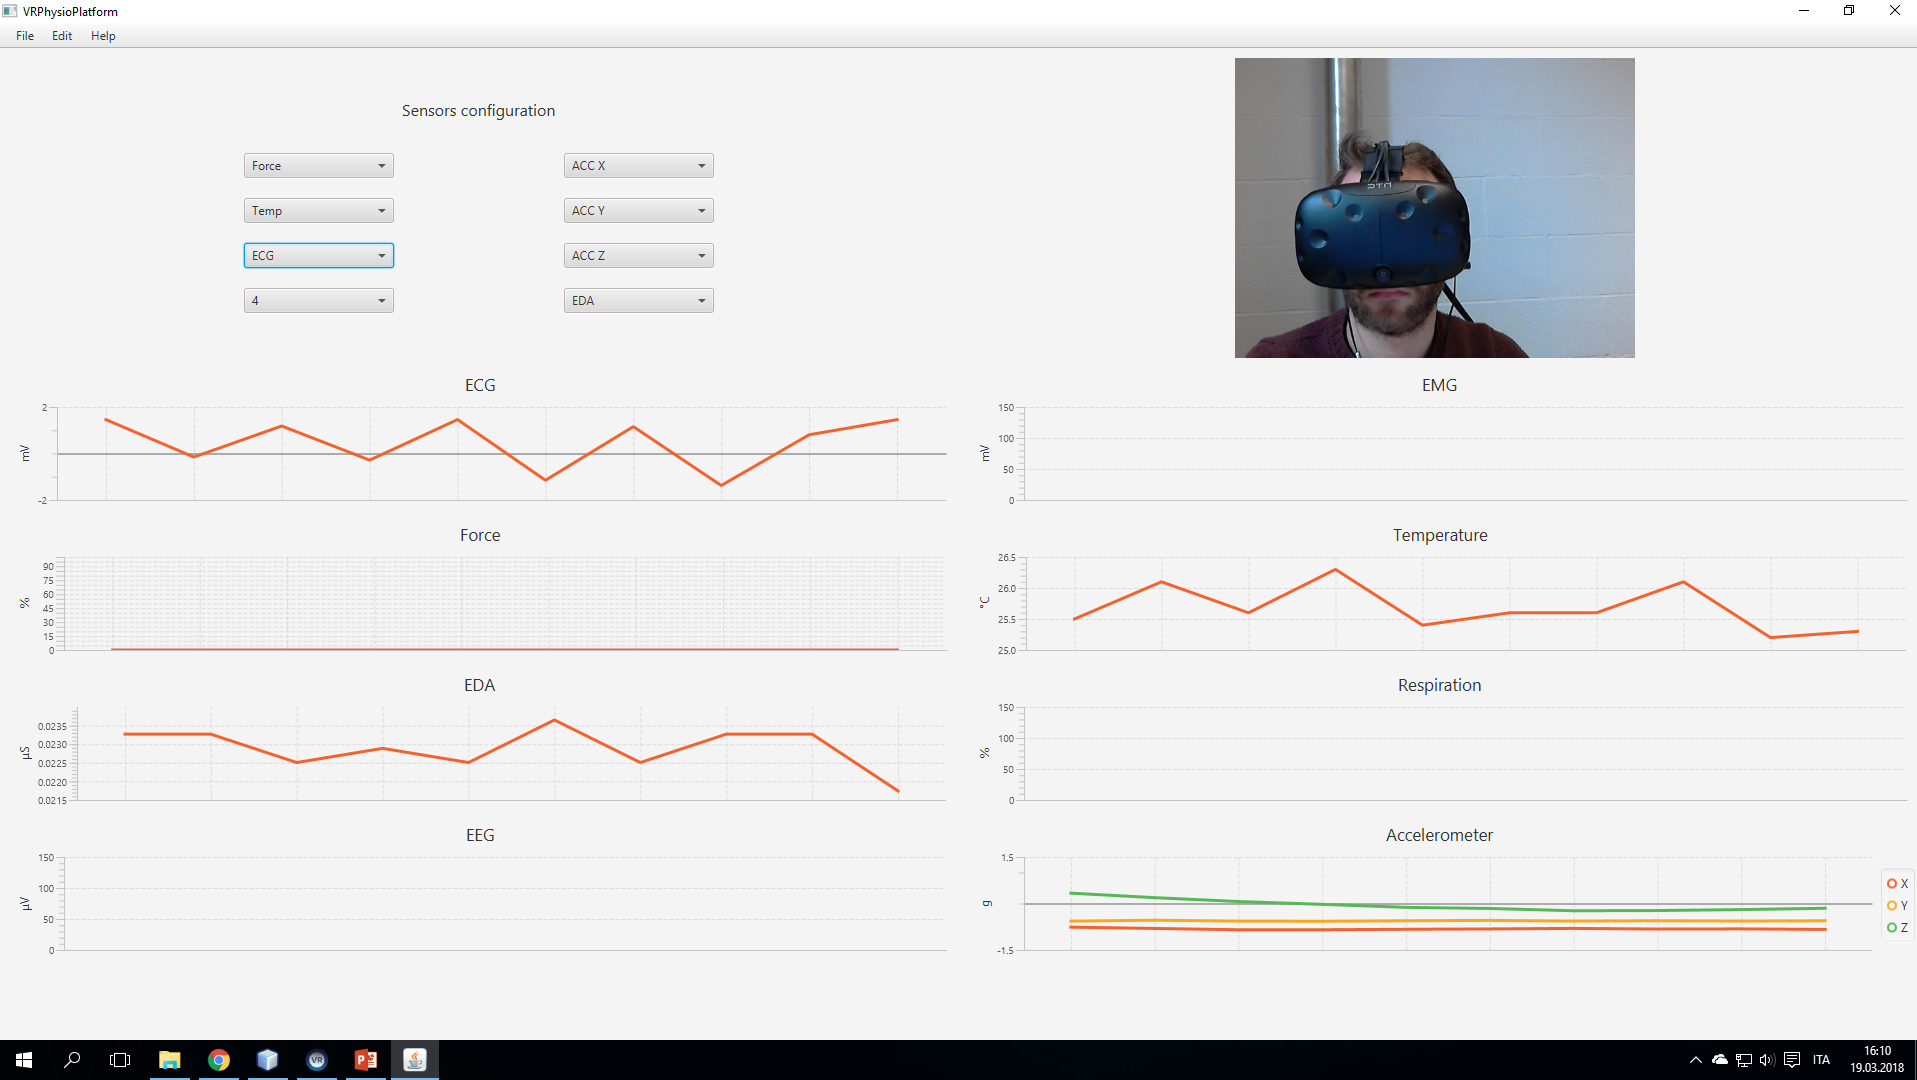
\includegraphics[scale=.45, angle=90]{images/realtime_complete1}
\caption{First prototype - Java application}
\end{figure}

\begin{figure}[p]
\centering
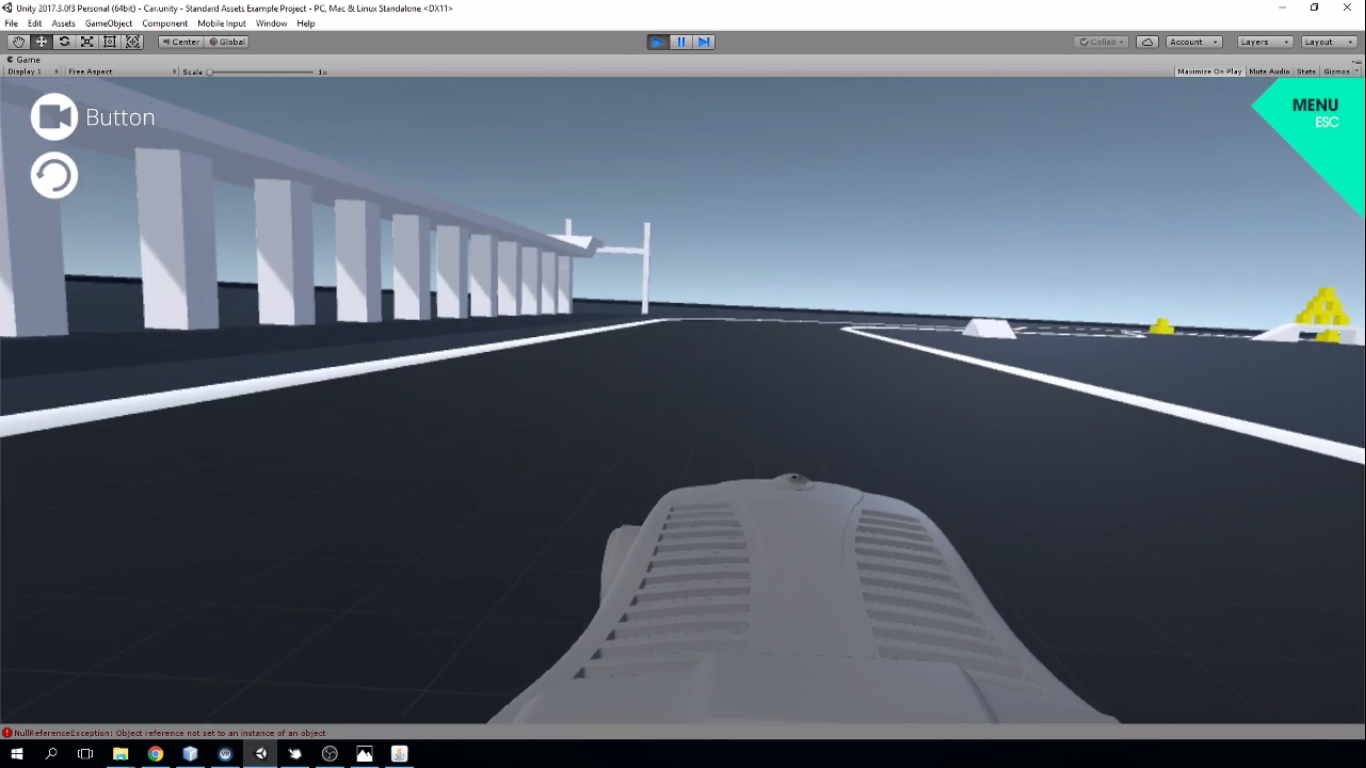
\includegraphics[scale=.45, angle=90]{images/realtime_complete2}
\caption{First prototype - Unity}
\end{figure}
\label{fig:prot1unity}


\subsection{Second prototype}
\label{subsec:secondprot}
The second prototype new functionality is the recording one. Once the examiner is able to see everything in real-time, he might want to record a session. In order to keep several over time, a new folder is created every time a new session is recorded. The folder contains camera video, physiological data and VR video, together with some text files containing synchronization information.
Following the same order as with first prototype, implementation started with camera.

\subsubsection{Camera}
As well as visualization, JavaCV library also provides recording functionalities. The class that handles recording is \textit{FFmpegFrameRecorder} which, as the name suggests, internally makes use of \textit{FFmpeg}. This is a complete and powerful software tool for recording, converting and streaming audio and video (see section \ref{sec:thirdparty}). 

For what concerns the user interface, a button was added to allow the examiner to start and stop the recording.
First we need to initialize a new recorder object specifying output path, video resolution and number of audio channels. After setting some other parameters, the recorder can be started. This happens when the user clicks the \textit{Start recording} button. In order to actually record a frame, we need to call the \textit{record(Frame frame)} method on the recorder passing as an argument the frame captured in prototype 1 (see code snippet 4.1). This method is called inside the \textit{CameraRunnable} class created before. A \textit{record} boolean was used to indicate when the recording is active.
After being recorded, the files need to be synchronized. The synchronization algorithm is the one illustrated in section \ref{sec:sync}. The information about the initial and final timestamps is written in a text file inside the directory of the current session. 
When the recording starts, the current timestamp is acquired through the \textit{System.currentTimeMillis()} function, which returns the difference, measured in milliseconds, between the current time and midnight, January 1, 1970 UTC. As said before, the granularity of the value depends on the underlying operating system: since we are operating on Windows 10, the value will have a 10 milliseconds accuracy. This is not a big deal because a few dozen delay in synchronization is undetectable by humans and therefore is definitely acceptable. Instead of the final timestamp, in the text file was stored the duration in milliseconds of the recording.
This metadata was saved as a JSON tree containing both camera and signals information. Camera fields were initial timestamp, duration (milliseconds), frame rate, size (kilobytes) and path of the file relative to the application main directory. Signals fields instead were initial timestamp, sampling rate, number of samples and path of the file relative to the application main directory. The following example shows the structure of the camera and signals metadata file.
\\
\begin{lstlisting}[caption={Recorded files metadata example}, captionpos=b]
{
	"cameraVideo":{
		"timestamp":1526219413241,
		"frameRate":30,
		"duration":160367,
		"size":19465223,
		"path":"\20180513_154834\cameraVideo.mp4"
	},
	"signals":{
		"timestamp":1526219413241,
		"samplingRate":1000,
		"samples":158671,
		"path":"\20180513_154834\signals.txt"
	}
}

\end{lstlisting}

Code snippet 4.4 contains portions of code that implement what stated above. For details about synchronization see section \ref{sec:syncrealization}.  
\\
\begin{lstlisting}[caption={Camera recording}, captionpos=b]
import org.bytedeco.javacv.FFmpegFrameRecorder;
...
private Timestamp timestamp;
private FFmpegFrameRecorder recorder;
private boolean record = false;
private static long startTime = 0;
...
recorder = new FFmpegFrameRecorder(
                cameraVideoPathTemp,
                captureWidth, captureHeight, 0);
recorder.setVideoCodec(avcodec.AV_CODEC_ID_H264);
recorder.setFormat(MP4);
recorder.setFrameRate(FRAME_RATE);
... // Additional recorder settings
... 
private void startRecording() {
	try {
		recorder.start();
		record = true;
	} catch (FrameRecorder.Exception ex) {
		logger.log(Level.SEVERE, "Error while starting camera recording", ex);
	}
}

private void stopRecording(){
	record = false;
	recorder.stop(); 
	...
}
..
class CameraRunnable implements Runnable{
	@Override
	public void run() {
		...
		if (record){
			startTime = System.currentTimeMillis();
			timestamp = new Timestamp(startTime);
        	...
			try {
				recorder.record(capturedFrame);
			} catch (FrameRecorder.Exception ex) {
				logger.log(Level.SEVERE, "Error while recording the frame", ex);
		}   
    }
}
        
\end{lstlisting}

\subsubsection{Physiological signals}
For recording physiological signals we can just extend the reading functionality presented above. Saving sensors data in fact is not hard, since data frames can be easily represented as strings, thus they can be written in plain text files. The idea is that when we acquire the signals (once every millisecond), instead of just plotting the value (every 100 milliseconds) we can write it on a file.  
The same \textit{record} flag as before can be used to control this behavior. If it is true then we can store the value, otherwise we just save it in a variable. Data frame is formatted as a tab-separated string containing sequence number, digital input flag and actual signals data.
Before writing the frames, we insert in the file a line containing signals metadata such as timestamp, sampling rate and, most importantly, names of the used sensors. This allows to know which specific sensor each column refers to and is also the reason why we need combo boxes to configure the signals channels. Ax example signals file is the one in figure 

\begin{figure}[h]
\centering
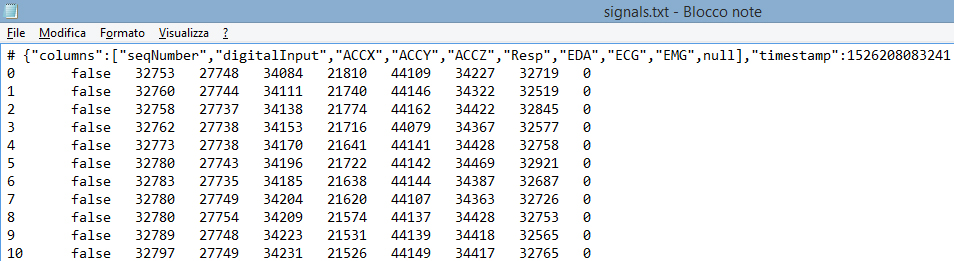
\includegraphics[scale=.41]{images/signals_file2}
\caption{Saved signals file example}
\end{figure}

Taking into account all these considerations, the signals recording code results as just an extension of the one reported in code snippet 4.2.
\\
\begin{lstlisting}[caption={Signals recording}, captionpos=b]
import java.io.FileWriter;
import java.io.IOException;
...
private FileWriter signalsWriter;
...
if (!devs.isEmpty()){
	try {
		signalsWriter = new FileWriter(signalsPathTemp);
	} catch (IOException ex) {
		logger.log(Level.SEVERE, "Error while creating signals writer", ex);
	}

	int[] counter = new int[1];
	Thread getSignals = new Thread(() -> {
		try {
			dev.GetFrames(1, frames);
			if (record){
				Device.Frame frame = frames[0];
				String output = counter[0] + "\t" + frame.dig_in + "\t";
				int length = frame.an_in.length;
				for (int j = 0; j < length-1; j++){
					output += frame.an_in[j] + "\t";
				}
				output += frame.an_in[length-1];
		
				signalsWriter.write(output + System.lineSeparator());
				counter[0]++;  
			}
		} catch (BPException ex) {
			logger.log(Level.SEVERE, "Error while getting the frames", ex);
		} catch (IOException ex) {
			logger.log(Level.SEVERE, "Error while writing signals data", ex);
		}
	});
}
        
\end{lstlisting}

\subsubsection{Unity}
For what concerns Unity VR recording, we can use the \textit{RockVR} plugin (see section \ref{sec:thirdparty}). It allows to record the visual output of the game or to send it to a streaming server. There are some customizable options such as output directory and frame rate, but to achieve the application's recording and synchronization goals there is the need of some adjustments. Basically we need the plugin to save the file inside the same session directory as the Java application and to write metadata such as initial timestamp and duration into a text file. The directory selection is an issue because we do not know if the examiner first starts the application or Unity. If he first starts the Java application, this has to create a new folder and Unity has to recognize and use it; if he first starts Unity, the opposite should happen. The solution was to use a "status" text file, placed in framework root directory, that contains the information about which application created the directory. In this way when the other one reads the file it understands that it must not create a new directory and it must use the already existing one. 

The recording functionality is obtained editing parts of some RockVR scripts in order to make the desired behavior possible. 
The scripts are written in C\# but, since they basically do the same things, the logic of the code is almost the same as the Java application one, so it is not explicitly reported in this section. Recording starts when the user presses the R key on the keyboard, timestamp is obtained using \textit{DateTime.UtcNow} and the metadata JSON file has the exact same structure as the "camera" one in code 4.4.

The general execution flow is the following: Unity starts and checks the "status" file, creating the directory if needed, then waits for the examiner to start the recording. When it happens, timestamp is saved in the text file and recording begins; at the end of the session duration and size are added to the file.

\subsubsection{Synchronization}
\label{sec:syncrealization}
Once the recording is stopped from both Unity and the Java application, the created files need to be synchronized. As explained in the design chapter, synchronization is based on system timestamps and files are cut according to timestamps difference. Here are presented some implementation details about it.

First of all, synchronization cannot be executed automatically by the framework at the end of the recording. The reason is that files take some time before being permanently and correctly saved on the hard drive, depending on the session length. This means that the synchronization phase cannot start immediately or after a fixed amount of time. The solution is to give the examiner the responsibility to start it by pressing a button: he has to check if the files are correctly saved and then he can start the process. 

Synchronization is realized through the command line software\textit{FFmpeg} (see section \ref{sec:thirdparty}). There exist some Java wrappers of it but their usage was problematic, so the program was used directly from command line using the \textit{Process} Java class. This allows to create a system process, launch it and wait for its completion. An FFmpeg distribution was downloaded and placed in the same directory as the Java application (see section \ref{sec:build}) so that it is always available.

For what concerns the actual synchronization, first the system reads the metadata files about camera and VR videos (camera and signals have the same timestamp), then it compares their initial timestamps and durations. Combining these two values we obtain four possible cases:

\begin{enumerate}

\item camera video starts first and lasts longer than VR video;

\item camera video starts first and lasts less than VR video;

\item VR video starts first and lasts longer than camera video;

\item VR video starts first and lasts less than camera video.

\end{enumerate}

Let us analyze the first case. If camera video starts before VR video we need to cut its first portion in order to make the two videos start at the same time. If camera file lasts longer than VR file we also need to cut its final portion: by doing that we obtain two videos that start and end at the same time, thus they are synchronized. The same cuts we make on camera can be applied to signals file, since they share the same timestamp and duration. This reasoning can also be applied to case 3 simply reversing camera and VR video. 
Case 2 (and therefore 4) is a little bit more complicated because we need to cut the first part of the camera video and the last part of VR video, since it lasts more.  
FFmpeg is executed on a separate thread so that it does not interfere with the main application behavior. Code snippet 4.7 gives an overview of the different cases.
\\
\begin{lstlisting}[caption={Cut video cases}, captionpos=b]
long cameraVideoTs = cameraVideo.get(TIMESTAMP).getAsLong();
long vrVideoTs = vrVideo.get(TIMESTAMP).getAsLong();
        
double vrVideoDuration = vrVideo.get(DURATION).getAsDouble();
double cameraVideoDuration = cameraVideo.get(DURATION).getAsDouble();

double diff;
        
if (vrVideoTs > cameraVideoTs){
	// camera video starts first
	diff = vrVideoTs - cameraVideoTs;
            
	double start = diff/1000; //seconds

	double cameraNewDuration = cameraVideoDuration - diff;
	if (cameraNewDuration > vrVideoDuration){ 
    	// 1. camera video starts first and lasts longer than VR video
               
		double end = vrVideoDuration/1000;
		try {
			Thread cameraVideoCut = new Thread(new CutVideo(CAMERA_VIDEO, cameraVideoPathTemp, cameraVideoPath, start, end));
			cameraVideoCut.start();
        ...
        cutSignals(start*1000, end*1000);
        ...
        } catch (Exception ex) {
			logger.log(Level.SEVERE, "Error while cutting camera video", ex);
		}
	}
	else {
		// 2. camera video starts first and lasts less than VR video
	}
}
else {
	// VR video starts first
	diff = cameraVideoTs - vrVideoTs;
            
	double start = diff/1000;

	double vrNewDuration = vrVideoDuration - diff;
	if (vrNewDuration > cameraVideoDuration){ 
		// 3. VR video starts first and lasts longer than camera video
		...
	}
	else {
		// 4. VR video starts first and lasts less than camera video
		...
	}
} 
\end{lstlisting}

Cutting the signals file is very easy. Since we acquired data with a 1 kHz rate we have a line for each frame and frame counter represents time (e.g. 12500 refers to 12.5 seconds). This means that, assuming the difference between the timestamps is \textit{diff}, we only need to read the file line by line, ignore the first \textit{diff} lines and copy the others on a new text file. Same thing can be done to the last part of the file.

For what concerns the actual video cut task, a Java process launching \textit{FFmpeg} was invoked. The process is created through the \textit{ProcessBuilder} class, passing as parameters the string arguments that make up the complete command: path of the command to execute, input and output files path, starting and ending points. The class also allows to redirect the process output to the NetBeans console, letting the developer debug the application.

The problem with video cut is that it takes time. The first attempt with \textit{FFmpeg} included the option \textit{-codec copy}. This is very fast because makes the program skip decoding and re-encoding of the stream, but it is not accurate with respect to seeking. Video files are in fact composed of a number of \textit{keyframes}, special frames that contain a whole image of the stream. Intermediate frames, those that are between two keyframes, only store changes from the previous keyframe and not the whole image. This means that we cannot cut a video between two keyframes without first decoding it, because the information is not complete. The first attempt tried to cut the video indicating a specific (up to milliseconds) start time and including the \textit{-codec copy} option. This resulted in a video cut from the previous keyframe, with a significant error. Videos can in fact contain one keyframe for each 4 or 5 seconds of the stream. The only possible solution to this issue was to remove the copy option and decode the entire video, thus considerably slowing down the whole synchronization phase. This obviously depends on the length of the recording session but was considered not excessively long, so the solution was actually adopted.
A progress bar was added to the GUI to inform the user about the completion of the synchronization job. Code snippet 4.8 shows the creation and the launch of the \textit{FFmpeg} process.
\\
\begin{lstlisting}[caption={Cut video process}, captionpos=b]
private String ffmpeg;
...
ffmpeg = workingDirectory + "\\ffmpeg\\bin\\ffmpeg.exe";
...
class CutVideo implements Runnable{
	private final String video;
	private final String videoPathIn;
	private final String videoPathOut;
	private final double start;
	private final double end;
	...  
	@Override
	public void run() {
		...
		try {
 			Process process = new ProcessBuilder(
				ffmpeg,
				"-i",
				videoPathIn,
				"-ss",
				String.valueOf(start),
				"-t",
				String.valueOf(end),
				"-y",
				videoPathOut)
				.redirectErrorStream(true).start();

			StringBuilder strBuild = new StringBuilder();
			BufferedReader processOutputReader = new BufferedReader(new InputStreamReader(process.getInputStream(), Charset.defaultCharset()));
			String line;
			while ((line = processOutputReader.readLine()) != null) {
				strBuild.append(line).append(System.lineSeparator());
			}
			process.waitFor();
			...
		} catch (Exception ex) {
			logger.log(Level.SEVERE, "Error while cutting the video", ex);
		}
	}
}
\end{lstlisting}

\subsection{Third prototype}
The third prototype adds the replay functionality to the system and brings it to its final version. The first thing to do is to implement the playback feature for camera and VR videos, then the one for the signals. Finally, we can add markers insertion functionality.
In order to replay a session we first need to switch to \textit{Offline mode}, then to open a folder containing the files. Both these tasks are executable through the application menu bar. 

\subsubsection{Playback}
Camera and VR video can be played using the \textit{MediaPlayer} class that provides the basic media controls such as play, pause, stop and seek. It works inside a \textit{MediaView} graphical object and it just needs the path of the file to open. 
We use a single slider to give the user a visual overview on the playback progress. If a point on the slider is clicked, media players seek the corresponding time on the videos, and signals charts do the same. These behaviors are realized through property listeners that bind slider to media players and signals. Code snippet 4.9 gives an example of what said above and refers to VR video; the code for camera video is exactly the same.

\begin{lstlisting}[caption={Play video}, captionpos=b]
import javafx.scene.media.Media;
import javafx.scene.media.MediaPlayer;
import javafx.scene.media.MediaView;
import javafx.scene.control.Slider;
...
private MediaPlayer vrMediaPlayer;
@FXML
private MediaView vrMediaView;
@FXML
private Slider slider;
...
private void openVrVideo(String path) {
	if (path != null) {
		File file = new File(path);
		Media media = new Media(file.toURI().toString());
		vrMediaPlayer = new MediaPlayer(media);
		vrMediaView.setMediaPlayer(vrMediaPlayer);
            
		vrMediaPlayer.totalDurationProperty().addListener(
			(obs, oldDuration, newDuration) -> 				
				slider.setMax(newDuration.toSeconds()));
		slider.valueChangingProperty().addListener(
			(obs, wasChanging, isChanging) -> {
				if (! isChanging) {
           			vrMediaPlayer.seek(Duration.seconds(slider.getValue()));
            }
		});
		...
	}
}
\end{lstlisting}

For what concerns physiological signals, it was used the same chart class as the one used for the \textit{Real-time mode}. In order to play data fast and make seek possible, the whole text file containing signals data is stored in a list variable. In the large majority of cases this load does not affect system responsiveness because signals file is not big. Obviously if the recording session becomes very long (e.g. two hours) there may be some problems. The playback of the signals itself is realized with the same logic as the real-time acquisition one: \textit{Timeline} class with 10 readings per second. The code is very similar to that in code snippet 4.3 so it is not reported here.

\subsubsection{Markers insertion}
The last thing to do is to implement the functionality that allow to insert a marker in a point of a session to denote an important event that occurred.

The idea is to save this information in a new text file as a \textit{(timestamp, name)} pair. In this case timestamps are not the same entity as before: they indicate the number of milliseconds elapsed since the beginning of the video (exluding pauses), i.e. the time instant in the session when the event happens. Markers information is stored in JSON format (see example below).

\begin{lstlisting}[caption={Markers file example}, captionpos=b]
{
	"markers":[
		{
			"timestamp":97361,
			"name":"Event1"
		},
		{
			"timestamp":10906,
			"name":null
		}
	]
}
\end{lstlisting}


When the user wants to add a marker he clicks a button, playback stops and the corresponding timestamp is saved. A dialog window appears asking the user to insert a name; if this field is left blank the event will have a \textit{null} name. The \textit{(timestamp, name)} pair is then written on the text file. The point on the GUI when the marker is added is denoted by a red rectangle; if the mouse pointer moves over it a tooltip with the name of the event appears, if the mouse clicks on it, slider value is set to that point value.

\begin{figure}[h]
\centering
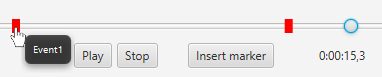
\includegraphics[scale=.8]{images/markers}
\caption{Markers appearance}
\end{figure}

Code snippet 4.10 shows the insertion of a marker on the GUI.
\\
\begin{lstlisting}[caption={Insert marker}, captionpos=b]
import javafx.scene.control.TextInputDialog;
import javafx.scene.control.Tooltip;
import javafx.scene.input.MouseEvent;
import javafx.scene.paint.Color;
import javafx.scene.layout.AnchorPane;
import java.util.Optional;
...
@FXML
private AnchorPane anchorPane;
...
@FXML
private void insertMarker(ActionEvent event) throws IOException {
	pause();
	int timestamp = (int)(slider.getValue()*1000);
	Marker marker = new Marker(timestamp);
	TextInputDialog dialog = new TextInputDialog();
	dialog.setTitle("Event name");
	dialog.setHeaderText("Insert event marker");
	dialog.setContentText("Name of the event:");
	Optional<String> result = dialog.showAndWait();
	result.ifPresent(name -> marker.setName(name));
	
	drawMarker(marker);
	
	... // add marker to markers list in the text file		
}

private void drawMarker(Marker marker){
	Tooltip tooltip = new Tooltip(marker.getName());
	Tooltip.install(marker, tooltip);
	marker.setFill(Color.RED);
        
	marker.setOnMouseClicked((MouseEvent event) -> {
		double value = marker.getOffset()*slider.getMax()/slider.getWidth();
		slider.setValue(value);
	});
	...
	anchorPane.getChildren().add(marker);
}

\end{lstlisting}




\section{Third-party software}
\label{sec:thirdparty}
During the design and realization phase several third-party libraries and tools were cited. They represent a big resource for developers because allow to reuse software written by others, often already tested and improved. Despite most of them were already mentioned earlier, here they are described in details.

\begin{description}

\item[SteamVR plugin] is a unity package that allows developers to integrate virtual reality into Unity projects. It is available for free on the official Unity Asset Store and works with both HTC Vive and Oculus Rift. 

\item[RockVR VR Capture] is a plugin for recording video and audio of virtual reality Unity applications. It also supports multi-camera captures and 360 video captures. Like SteamVR plugin, it can be downloaded for free from the Unity Asset Store and works with both HTC Vive and Oculus Rift.

\item[JavaCV] is a utility that wraps commonly used libraries for computer vision such as OpenCV, FFmpeg, OpenKinect and others. Its source code is available on GitHub and it can be automatically downloaded with Maven.

\item[Plux API] is the official BiosignalsPlux API and allows to connect to the sensors and retrieve data. Besides Java, it is also available for C++, Python, C\# and MATLAB, as well as Android and iOS. It can be obtained for free from the producer's website.

\item[FFmpeg] is one of the most famous and widespread frameworks for audio and video coding, decoding, filtering, streaming and playing. Its main component is a free and portable command line tool compatible with the majority of operating systems.

\item[Gson] is a Java library developed by Google for converting Java objects into their JSON representation. Its source code is available on GitHub and it can be integrated in a project using Maven.

\item[JSON Object] is a class representing the C\# equivalent of Gson. Its code is available on GitHub but it can be directly downloaded from the Unity Asset Store.

\item[Metadata extractor] is a Java library for reading and extract metadata from image and video files. It supports a variety of standards such as Exif, XMP and IPTC but also formats like WAV, AVI, MP4, PNG, GIF. It can be downloaded with Maven. 

\item[Java MP4 Parser] is a Java API for reading, writing and creating MP4 containers. It is able to mux audio and video, append recordings, change metadata and cut videos. The library can be retrieved through Maven.

\end{description}


\section{Build and usage instructions}
\label{sec:build}
Once the development phase is completed, we need to build the application so that it can be deployed and used by other people. Since it is composed of two modules, the system will be distributed as a Windows installer that installs the Java application and a Unity package that can be imported and used inside a Unity project.

\subsubsection{Java application}
The application uses some Maven dependencies that we need to include in the output \textit{jar} file. This can be done using the \textit{Maven Shade Plugin}, which allows to create a jar package containing also all the dependencies. 
After this step, we need to be able to launch the package as a regular desktop application. The tool we can use for this purpose is \textit{Launch4j}, a cross-platform tool for wrapping Java applications distributed as jars into Windows executable files (.exe). It also allows to add Java Virtual Machine (JVM) options, so that we can pass parameters to the execution of the program. We exploit this opportunity to specify to the JVM the path of the Plux dll file with the command \textit{-Djava.library.path=./lib}. This folder needs to be distributed together with the executable file. Once the .exe file is ready, we need to create an installer that installs the program on the user's computer. This operation can be done using \textit{NSIS} (Nullsoft Scriptable Install System), a tool used to create Windows installers from ZIP archives. Therefore we add the previously built executable file and the library folder to a new archive, together with the \textit{ffmpeg} folder containing the software for video cut. We import the archive into NSIS and specify the default installation folder. The output of the tool is a self-extracting executable file that can install the framework very quickly and easily.
The detailed steps to create the installer are the following:

\begin{enumerate}

\item build from NetBeans using the Maven Shade Plugin;

\item open the Jar file from step 1 into Launch4j and specify the output name;

\item inside the JRE tab, write 1.8.0 in the "min JRE version" field and a big number in the "max JRE version" field, since the app is not limited to run below a certain JRE version;

\item inside the JRE tab, write \textit{-Djava.library.path=./lib} in the "JVM options" field;

\item build the wrapper;

\item create a ZIP archive with the executable file of step 5, the \textit{lib} folder and the \textit{ffmpeg} folder;

\item run NSIS and select "Installer based on ZIP file";

\item open the ZIP of step 6 into NSIS, specify an installer name, select "\$PROGRAMFILES\textbackslash YourNameHere" in the "Default folder" field and insert a name;

\item generate the installer file.

\end{enumerate}

\subsubsection{Unity package}
The Unity package contains the SteamVR asset, the modified RockVR plugin, the JSON Object asset and some additional configuration files. Building the package is a trivial task because it can be done in the editor itself (select all the assets to include, right click on them and select "Export Package...").

When a user wants to use the package he has to import it and set some parameters in order to make it work properly. They basically consist in attaching video capture scripts to some game objects and adjust some of their properties. 
In the following list of required steps we assume that the right controller is used to control the recording but this can be changed without any constraints by the user.

\begin{enumerate}

\item import the package;

\item delete the \textit{Main Camera} object;

\item place the \textit{CameraRig} prefab (SteamVR/Prefabs) in the scene; 

\item place the \textit{CaptureCamera} prefab (RockVR/Vive/Demo/Prefabs) under \textit{CameraRig/Camera (head)}; 

\item attach \textit{Properties} file to a fixed game object (e.g. \textit{CaptureCamera});

\item attach \textit{CameraSampleCtrl} script (RockVR/Vive/Demo/Scripts) to \textit{CameraRig/Controller (right)}; 

\item attach \textit{Vive\textunderscore EventCtrl} script (RockVR/Vive/Scripts/Controls) to \textit{CameraRig/Controller (right)};

\item attach \textit{VideoCapture} script (RockVR/Video/Scripts) to \textit{CameraRig/Camera (head)/CameraCapture};

\item attach \textit{AudioCapture} script (RockVR/Video/Scripts) to \textit{CameraRig/Camera (head)/CameraCapture};

\item in the \textit{CameraRig/Controller (right)} inspector go to \textit{Video Capture Ctrl}, set \textit{Video Captures} size to 1, drag and drop \textit{CaptureCamera} into \textit{Element 0} and also into \textit{Audio Capture}.

\end{enumerate}

At this point Unity is ready to record sessions alongside the Java application.


\chapter{Validation}
The last chapter of this thesis is about the validation of the developed framework. The basic definition of software validation is to check if the final product meets customer's requirements and expectations. In this case requirements refers to high-level requests, i.e. general ideas and customer needs behind the product. This means that validation checks if software is compliant with what the stakeholders (investors, managers, users) asked. It only covers the basic concept of the product, it does not concern low-level specification or software performance.

The validation phase is generally executed after verification, which can be considered as the complementary process of validation. While validation concerns high-level requirements, verification deals with specification details and software behavior. We can say that it checks if the product is correct, i.e. if the software fully satisfies the requirements, if it contains errors or bugs, and so on. 

We can refer to this thesis project to make an example about the difference between the two concepts. Validation is about checking if the general idea of the framework is satisfied. The high-level requirement of this system is to make research work about VR and physiological signals easier by providing a ready-to-use environment that records and synchronizes the different streams. Moreover, the system should be a useful tool for easily find correlations between VR events and physiological signals. Another high-level requirement for the system is that it has to be user-friendly and easy to use also for users not expert in computer science.
The main validation task is therefore to answer the questions: \textit{is the system really useful to the potential users? Can we really have everything recorded and automatically synchronized? Can we really find with ease correlations and connections between what happens in VR and how the body reacts? Is the system easy to use by everyone?}

On the other hand, verification deals with checking if system requirements are satisfied. With this framework researchers can see in real-time, record and replay an experiment session; they can easily find in all the three sources (camera, VR and signals) key moments when events happened and mark them; they can access and analyze data with third-party tools. The questions we need to answers are therefore: \textit{can we see in real-time and record the session? Does synchronization work properly (errors, delay, etc)? Can we mark events? Does the system save data in a convenient format so that it can be properly analyzed?}

Although verification is an important step of software development, this chapter only focuses on validation. There are several methodologies that can be used to evaluate the validity of a system. In the next sections are presented two different techniques that can be considered as parts of the validation process. The first one is a \textit{proof of concept} test and the second one is a \textit{usability} test. 

\section{Proof of concept}
A proof of concept is a realization of a certain idea to prove its effectiveness and validity. It is often used to demonstrate that a theory is feasible or that a system behaves correctly; it may be represented by a prototype, a demo, a partial system, and so on. A proof of concept can be also used to show that a system satisfies the requirements and expectations it was designed for. The latter case is the one this proof of concept refers to: we will design a scenario that will demonstrate the potential of the system and that can be a good measure for validation. In particular, the proof of concept will allow to answer the question about the possibility to find correlation between VR events and body reactions. Obviously physiological signals data and correlation can be analyzed also without the framework. Body signals are independent from the context, their acquisition does not depend on the virtual experience and their analysis can be conducted offline with any suitable software. However, a more complex task is to relate data with events that happen in VR. In some cases it would not be easy to associate a point in the data to each relevant event because the streams are not synchronized. This especially applies if acquired physiological data is large enough, i.e. the recorded session is very long.

The main advantage of the framework is just that: to facilitate research work and analysis with a system that handles recording and synchronization. Using the framework allows to replay a session, find the events by watching the videos and mark them, allowing an offline analysis of the data with the exact knowledge of when things happened.

In order to prove that the system is actually helpful for the above purpose, the proof of concept will be constituted by a virtual experience in which an event happens. During the experience physiological data will be acquired and at the end of the session the streams will be synchronized. Finally, data will be analyzed showing that it is easy to find relevant moments and draw conclusions about the whole experience.

\subsection{Design and development}
The proof of concept idea was to create a VR scenario containing an event that could generate clearly visible reactions in users. In this way we would be able to say for sure if event and body response are correlated. There exist a lot of different human emotions that can arise as a response to external events and stimuli. Some of them are easily measurable with physiological signals, others are harder to detect. Since we need unambiguous results, we can exploit a well-studied emotion: fear. We know that fear causes several physiological reactions and in particular heart rate acceleration and respiration and skin conductance increase  \cite{levenson1990voluntary}. Furthermore, a loud auditory stimulus can make muscles contract as a consequence of a startle response. The muscle that reacts more quickly to this kind of stimuli is the sternocleidomastoid \cite{brown1991new}.

Starting from these considerations, the proof of concept scenario will involve a frightening visual stimuli coupled with a very loud noise. In particular, the virtual environment will consist of an abandoned dungeon with some rooms and corridors. In one of the rooms there is a monster that only appears when the player goes inside: as soon as the player enters the room a frightening loud scream starts and the monster appears and moves towards the player very fast; when it reaches him, it disappears. This scenario should allow to register a clean physiological signals difference between what happens before and after the event. 
With respect to what said above we will measure heart rate, electrodermal activity (EDA), electromyography (EMG) and respiration. In addition to these signals we will also collect body acceleration with an accelerometer.

Going more in depth with the VR scene, it is developed in Unity ising only free assets found on the internet. The main scenario consists of a dungeon package named \textit{Decrepit Dungeon LITE} while the monster is part of the \textit{Fantasy Monster (Wizard) DEMO}; both these packages were downloaded from the Asset Store. 

\begin{figure}[h]
\centering
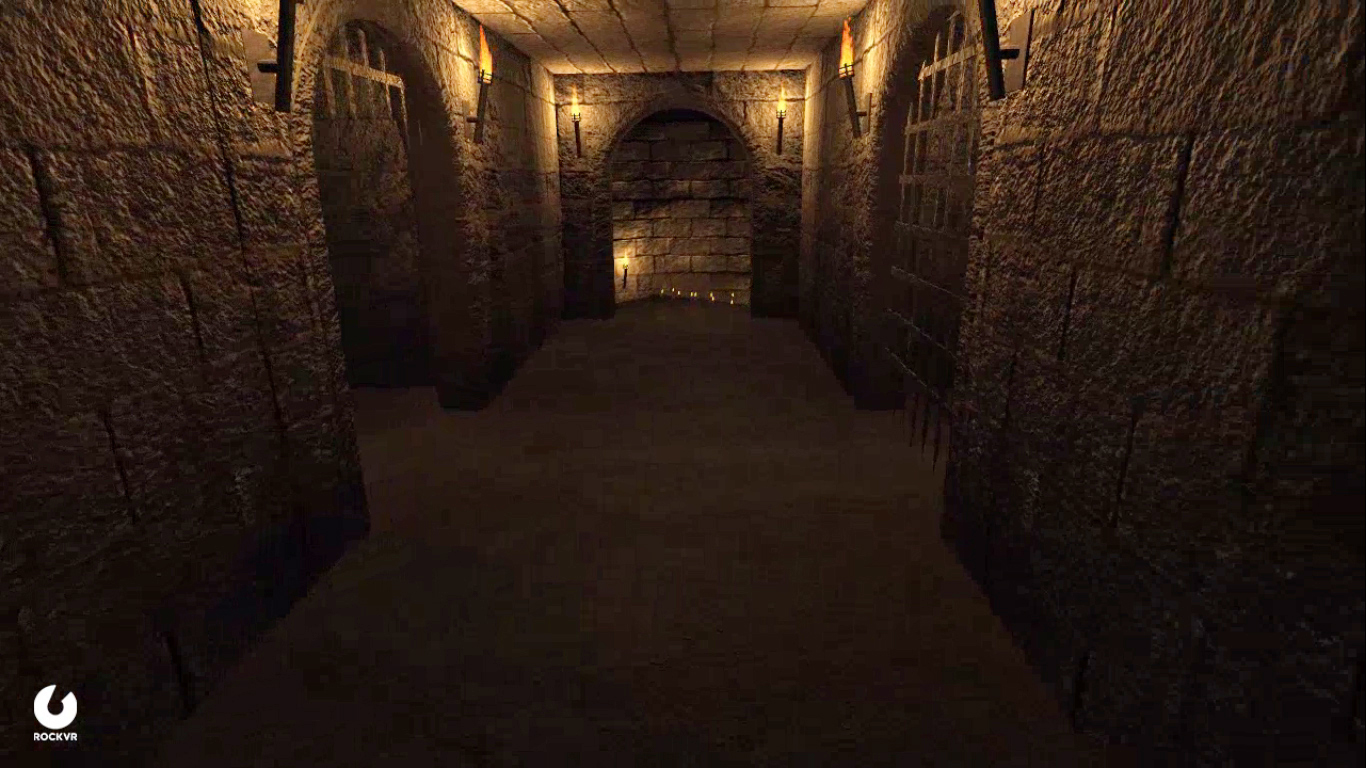
\includegraphics[scale=.28]{images/dungeon2}
\caption{Dungeon scene}
\end{figure}

Locomotion is a crucial aspect in VR games. Developers usually avoid classical first person walking because it often causes sickness in players (see section \ref{sec:measures}). The most secure way of implementing locomotion without generating sickness is through pointers: player uses the controller to point a spot in the environment, pressed a button and the character is teleported there. Although this solution usually avoids sickness, in this proof of concept scene it is not the best option. Players need to walk through the corridors and enter rooms in order to explore the whole environment and to finally meet the monster. Simply teleporting into the designated room would not produce the same scary effect. Another reason why in this case sickness is not a big issue is that the experience should be very short: since the dungeon environment is quite small, people should not a lot of time to complete the test. Locomotion is achieved using \textit{Virtual Reality Toolkit} (VRKT), a collection of tools and methods for rapidly developing VR projects. It includes a locomotion system that makes the character move using the HTC Vive controller touchpad. The package also include some demo scenes where the players can get learn and get used to the locomotion system.

\begin{figure}[h]
\centering
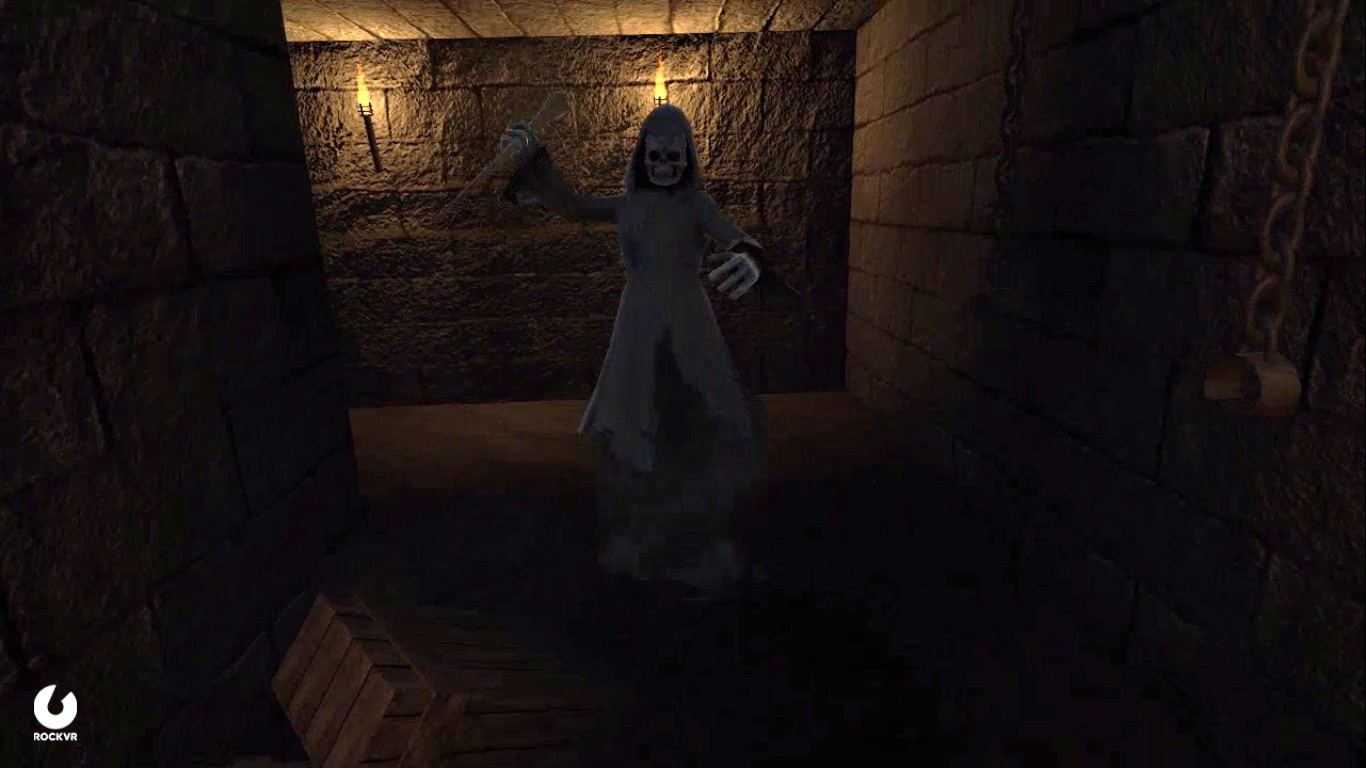
\includegraphics[scale=.28]{images/monster2}
\caption{Monster}
\end{figure}

The experiment is conducted in such a way that participants are focused on exploring the environment and do not expect a scary event. In order to achieve this goal, we say them they have to find a key that is placed in a specific room in the shortest possible time. Finally, audio is used to create an even more immersive and challenging experience: players can ear the character's footsteps while it walks and a background music plays during the whole experience. The selected music track is \textit{Find Your Way}, extracted from \textit{Final Fantasy VIII} original score. This track should engage players and make them feel like they are in a challenging quest. Finally, the frightening noise was a scary scream found on the internet.


\subsection{Test protocol}
The test was conducted on 15 volunteers, 10 males and 5 females, aged between 19 and 38 (mean 26.27, SD 5.33). They were asked if they had experience with VR, videogames or a touchpad controller. The majority of them had experience with videogames, tried VR once but had no experience at all with touchpad controllers. Participants signed a consent form about being filmed and being aware of possible VR sickness.
In order to be rigorous and formal, the test was conducted in the exact same way for every participant. The test protocol is the one that follows. For each step is indicated the estimation of its duration. Each session should take 20 to 25 minutes.


\begin{enumerate}

\item Inform the participant about the test: it will be a VR scene, we will collect his physiological signals during the experience and we will record both the VR video and the participant's face with a webcam (3 minutes);

\item let the participant fill the consent form (2 minutes);

\item collect participant's data: age, sex, experience with VR, experience with videogames and with touchpad controllers (2 minutes);

\item describe the VR scene to the participant(30 seconds): 
\begin{quote}
"You are in a dungeon of a castle and you have to find a key in the shortest possible time. The key is clearly visible once you reach the room where it is placed; you can just walk on it in order to get it"; \end{quote}

\item describe the locomotion system to the participant (30 seconds):
\begin{quote}
"You can look around simply turning your head and you can walk using the controller touchpad. The reference for the locomotion is the headset direction, i.e. pressing on the positive Y axis will make you move forward with respect to the direction you are facing";
\end{quote}

\item set up the sensors on the participant's body (5 minutes):
\begin{itemize}
\item Accelerometer, placed on the chest through an elastic band;
\item Respiration, placed on the abdomen through an elastic band;
\item EDA, placed on the left hand index finger and middle finger;
\item ECG, placed on the left side of the chest, below the heart;
\item EMG, placed on the neck, on the sternocleidomastoid muscle;
\end{itemize} 

\item let the participant play an example VR scene (from VRTK example scenes) in order to get used to VR and locomotion system (3 minutes);

\item check if all the sensors are working properly through the official BiosignalsPlux application (OpenSignals) (30 seconds);

\item prepare the test (1 minute): 
\begin{itemize}
\item check if the Java application task is still running from previous tests (if yes, kill it);
\item check if HTC Vive headset and controllers are ready;
\item check if physiological signals hub is turned on;
\item check if "status" file is correct;
\end{itemize}

\item run the system (1 minute):
\begin{enumerate}
\item run the Java application;
\item configure sensors inside the application;
\item check if signals are correctly acquired;
\item start recording from the application:
\item play the Unity scene;
\item start recording from Unity;
\end{enumerate}

\item let the participant play the VR scene until he finds the key, then wait 30 seconds more (2 minutes);

\item stop recording (30 seconds):
\begin{enumerate}
\item stop recording from Unity; 
\item stop recording from the Java application;
\item check if everything went fine;
\item stop the Unity application;
\end{enumerate}

\item synchronize videos and signals (1 minute);

\item unplug sensors from the participant's body (30 seconds);

\item tell the participant not to say anything about the experience to other people (30 seconds).

\end{enumerate}

\subsection{Results}
Every session was successfully recorded and synchronized. The first thing done was to plot data on a chart to see if everything went well (figure 5.3). Due to sensor placement problem, acquired respiration data was not clean and therefore not meaningful for the experiment results.
The other collected measures were good enough so it was possible to proceed with analysis. If we exclude respiration we have four signals to analyze - accelerometer, EDA, ECG and EMG. Data was studied starting from the knowledge of when the frightening event occurred. This was easily achieved through the offline mode of the application by replaying the whole session, finding the event moment and marking it.

Another technique that can be used to identify with accuracy when the event happens is to use EMG and accelerometer data. Since accelerometer was placed on the chest, it should not move much during the VR experience if there are no relevant events; on the contrary, if something scary happens (monster and loud scream) the body reacts with a small and sudden move - the so-called jump scare. This movement can be easily detected looking at accelerometer data. The same concept applies for EMG. During the experience muscles are generally relaxed, they only contract as a response to sudden stimuli like a loud noise. 
Therefore the idea was to analyze both accelerometer and EMG data in order to find the max (or min) value of the session: these values should correspond to the very moment when the event occurred. 
With the purpose of showing that this idea works, we made a comparison between event timestamp registered through replaying the session and the one registered through data analysis. Since the replaying technique is based on a human research of the right timestamp, it cannot be very accurate; data analysis instead has milliseconds accuracy. We consider successful a comparison that shows a difference of at most 1 second between the two techniques. 

\begin{figure}[p]
\centering
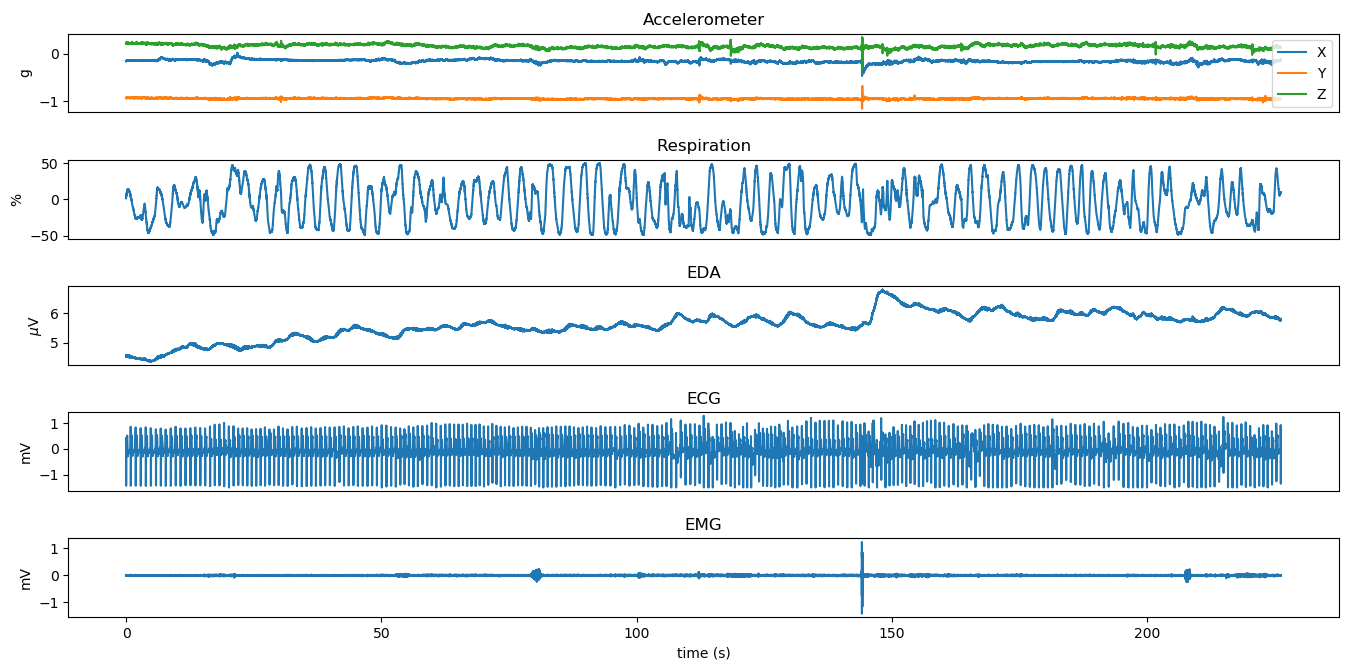
\includegraphics[scale=.68, angle=90]{images/plot}
\caption{Data plot example}
\end{figure}

Another thing that has to be taken into account is that there can be noises in the signals or unexpected sudden movements by the participant without any event, for example VR headset problems, cable stuck, sickness. Since accelerometer signal is composed of three axis data, we have four total data sources: we consider the comparison successful is at least three of them report the same value as the one registered in the offline mode.

Of the 15 sets of data we have, 8 resulted in the same value for manual analysis and for all four data channels, 3 for manual analysis and three data channels, 1 for manual analysis and only one data channel and 3 presented totally different values. For the success criteria stated above we can say that 11 out of 15 samples resulted successful with respect to comparison.

The other relevant measures we acquired are ECG and EDA. They are not helpful to determine the event timestamp because they do not present significant changes in the exact moment it happens. They instead should tend to gradually change after the event occurs: in our specific case they should increase. 
Hence the idea was to see if they actually change before and after the event in order to find out if there is any correlation between event and body reaction. The choice was to examine mean heart rate and EDA in the 30 seconds preceding and following the event. More specifically, since the event can cause sudden movement that affects the measurement, first 3 seconds after the event were skipped and the mean was computed for the subsequent 30 seconds. EDA signal was ready to be analyzed but ECG was not. We were interested in mean heart rate, so we needed to extract this value from the ECG signal. This was achieved through the \textit{Python Heart Rate Analysis Toolkit} \cite{vanheart}, a framework for heart rate analysis in Python that allows to extract heart rate from ECG and to plot the data. The toolkit analyzes the peaks of the signal, rejects the incorrect ones and computes heart rate. Figure 5.4 shows an example with a 30 seconds ECG.

\begin{figure}[h]
\centering
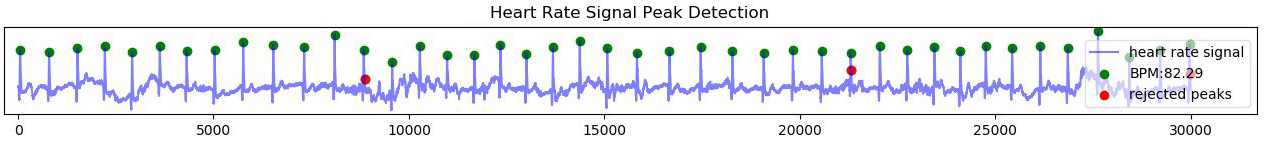
\includegraphics[scale=.419]{images/peaks0}
\caption{Heart rate from ECG}
\end{figure}

Because of noisy signal, the toolkit was not able to extract heart rate from 4 of the 15 acquired ECGs, so they were discarded. From each of the remaining 11 signals were extracted two portions of 30 seconds each, the first one starting 30 seconds before the event and the second one starting 3 seconds after. Heart rate was derived from the two portions of each signal and then the difference between them was computed. The average heart rate difference between before and after the event was 12.32\%. 
% why 30 seconds before: relaxed and used to the vr experience

Finally, EDA data was analyzed. In this case the acquired signal had no problems so every acquired data was correctly analyzed. As heart rate, average EDA was computed for two parts of the original stream: 30 seconds before the event and 30 seconds right after it (EDA is not influenced by movements so there was no need to skip the first 3 seconds after the event). After this, difference between the two portions was computed and it resulted to be 10.17\%. 

\subsection{Discussion}
Starting from the comparison between "manual" and data-driven approach to find the event in the recorded session, we found out that 11 out of 15 cases resulted successful. This result leads us to conclude two things. The first one is that once the session files are synchronized, identifying the event time is easy. The only thing to do is to replay the session, find the event and mark it. The second outcome is that data analysis allows to find easily detectable events in the majority of cases, and that it brings us the same results as the manual analysis. This system feature is therefore useful to the potential users because it allows to facilitate the general analysis process by easily finding key events of the experience.

For what concerns ECG and EDA analysis, it confirms the idea that body reactions to events are clearly visible is we know when the event happens. This means that there is a correlation between them and that this correlation is easily analyzable using the framework.

\section{Usability test}
A usability test is a technique used in user-centered design to understand if a product is easy to use testing it on real users. It is usually conducted letting users complete some task and observing their performances. 
This can include recording the test, measuring the time taken to complete the task, counting the errors made during the task, ask questions to the user, collect suggestions and measure any other kind of potentially useful parameter. Usability test are often conducted on prototypes of the system, so that with the results of the test developers can improve the prototype and meet users needs and suggestions. 

In our case the system was tested with several methodologies, starting with letting the users perform tasks and measuring the time they take for completing each task. This part of the test was divided into two sections, one for the real-time mode and one for the offline mode. The latter was one of the most important parts of the whole validation phase because it could allow to determine if having the session synchronized is actually useful. In particular, the offline mode part of the usability test was divided in two tasks: the first one's goal was to find the moment when the event occurs by manually inspecting the three original non-synchronized sources (VR video, camera video and signals); the second one's goal instead was to find that moment using the framework offline mode (with a different recorded session). 
By comparing the two tasks times we could determine whether the application can actually be helpful for finding easier and faster the key moments of the session.

After these tasks, users were asked to answer general questions about system functionalities: this phase was useful for understanding if users could think of different approaches for synchronizing files or for analyzing data.
The last step of the test was to let users fill a questionnaire about general usability of the system. The used questionnaire was the \textit{System Usability Scale} (SUS) \cite{brooke1996sus}, a scale developed by John Brooke in 1986 and become a standard in this type of tests. It gives a final score from 0 to 100 and the average value is 68, so any value above this number is considered good. The scale is reported in figure 5.5.

\begin{figure}[p]
\centering
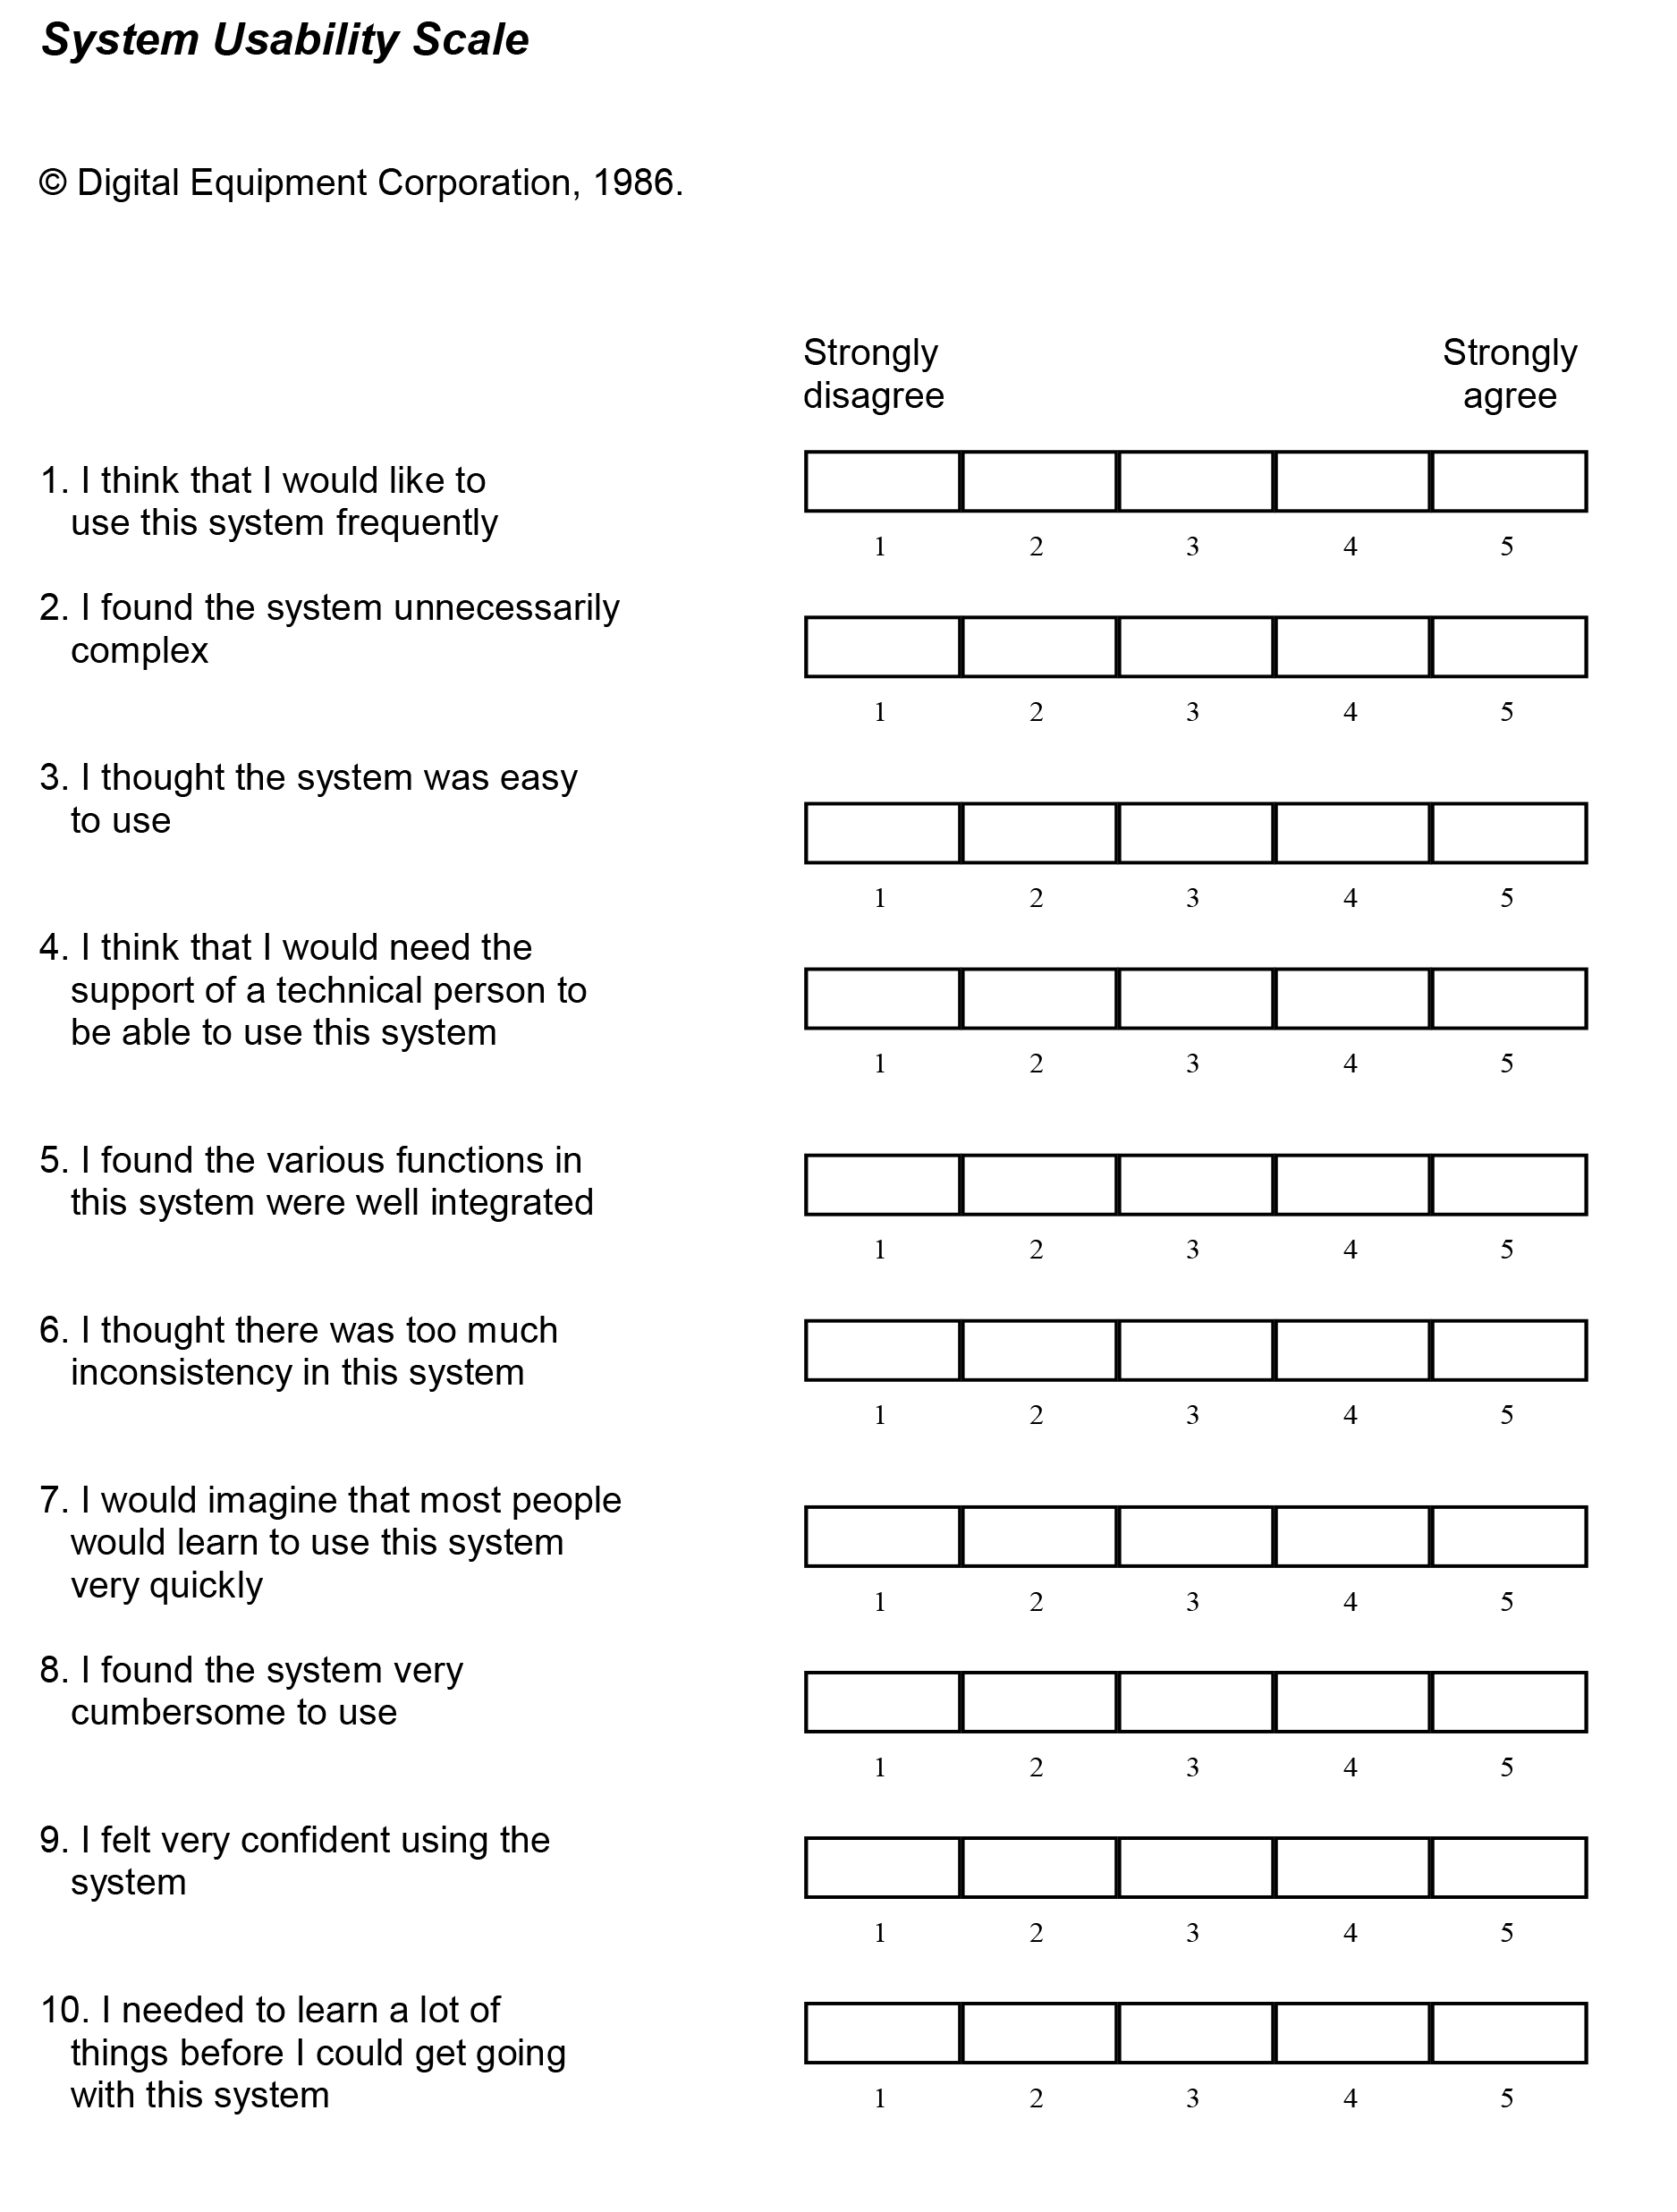
\includegraphics[scale=.92]{images/sus}
\caption{System Usability Scale}
\end{figure}

\subsection{Test protocol}
This section presents the detailed protocol used to perform the tests. The first requirement for this test was to use non-expert users, i.e. people that are not experts in data recording and analysis. The reason behind this choice was that the potential target users of this framework are represented by researchers that might not have any experience with this kind of functionalities. In this way we wanted to figure out if non-experts people could actually use the system. The first step of the test was therefore to collect participants' data such as age, sex, education/professional training and expertise in the system main functionalities. After that, a video tutorial was showed to the users in order to make them understand the basic functionalities of the system. It showed how to run the Java application and the Unity scene, how to configure the sensors, how to start, stop and synchronize a recording session, how to switch to offline mode, how to open a previous recording, how to play it and how to add a marker to it.

After watching the video, participants were allowed to ask questions about anything they did not understand, then they started the test and had to complete the assigned tasks. The first one was to simply configure the sensors inside the application, start a recording and stop it after an event happens. The used scene was the dungeon one from the proof of concept; the event was the appearance of the monster, that occurred 10 seconds after the recording started. 

The second phase was composed of two tasks. The first one was about finding the event in a previously recorded non-synchronized session looking inside the three files one by one. The second one's goal was the same as the other but using the application with a different recorded session. The two tasks were executed in a random order to be sure they did not influence users. After each task the user was asked about the data graphs, both inside the application and using a provided Excel plot of the data. The purpose of these questions was to understand if non-experts users were able to understand basic plots and to read data from them.

The test was conducted on 15 people, 9 males and 6 females, aged between 19 and 38 (mean 26, SD 5.41); 13 of them were computer engineers or computer science students, 1 was a mechatronic engineer and 1 was an educational science student. The complete test protocol is the following:

\begin{enumerate}

\item collect the participant's personal data: age, sex, education/professional training;

\item ask for expertise - on a scale of 1 to 5 (1 for no experience, 5 for expert) in the following topics:
\begin{itemize}
\item data analysis;
\item physiological data recording;
\item virtual reality system use and setup;
\item programming;
\end{itemize}

\item let the participant watch the video tutorial;

\item the participant can ask the examiner questions about things he did not understand from the tutorial;

\end{enumerate}


\subsubsection{Phase 1: Real-time mode}    

\begin{enumerate}

\item the participant is given the sensors connected in the following way:

\begin{enumerate}
\item ECG;
\item Respiration;
\item EDA;
\item Temperature;
\end{enumerate}

\item \textit{Task 1.1}: 

the participant has to run the Java application, correctly configure the signals and start a recording; time measurement starts when the application window is displayed and ends when the recording starts;

\item \textit{Task 1.2}: 

the participant has to run the Unity scene and start a new recording; time measurement starts when the scene is loaded and ends when the recording starts;

\item \textit{Task 1.3}: 

the participant has to wait for the event to happen, stop the recording from both the Java application and Unity, wait for the VR video being successfully created and stop the Unity scene; time measurement starts at the end of Task 1.2 and ends when the Unity scene is stopped;

\end{enumerate}

\subsubsection{Phase 2: Offline mode}    

\begin{enumerate}

\item the participant is given the Java application and two already recorded sessions of the proof of concept test (the dungeon with the monster), i.e. two folders with camera video, VR video and signals; only one of the sessions is already synchronized;

\item examiner tosses a coin to determine if the participant has to first perform Task 2.1 or Task 2.2;

\item \textit{Task 2.1}:

the task goal is to open the folder from the Java application, replay the session and insert a marker (with any name) in the point where the monster appears; time measurement starts when the application window is displayed and ends when the user correctly inserts the marker;

\begin{itemize}

\item \textit{Question 2.1.1}: In the moment when the event happens, is the EMG value out of the range [-0.1, 0.1] mV? [Correct answer: \textit{Yes}]

\item \textit{Question 2.1.2}: In the moment when the event happens, is the respiration value out of the range [-40\%, 40\%]? [Correct answer: \textit{No}]

\end{itemize}

\item \textit{Task 2.2}: 

the task goal is to open the non-synchronized folder from the file explorer and find the moment where the monster appears in these 3 files (in this order): 
\begin{enumerate}
\item \textit{vrVideo\textunderscore TEMP.mp4}, pausing the video in that moment;
\item \textit{cameraVideo\textunderscore TEMP.mp4}, pausing the video in that moment;
\item \textit{signals.xlsx}, clicking on the graph point;
\end{enumerate}

time measurement starts when the participant opens the folder and ends when he correctly identifies the point on the graph;

\begin{itemize}

\item \textit{Question 2.2.1}: After a few seconds from the event, does the EDA reach the value 12? [Correct answer: \textit{No}]

\item \textit{Question 2.2.2}: In the moment when the event happens, is the accelerometer Z axis out of the range [-0.2, 0.4]? [Correct answer: \textit{Yes}]

\end{itemize}

\item participant fills the \textit{System Usability Scale} questionnaire;

\item participant is asked the following questions: 

\begin{itemize}

\item (Showing him the content of a signals txt file)
Would you be able to plot a text file containing raw signals data like these? If yes, how? 

\item How would you perform the research to find the point where the monster appears in the different files? Would you have a different technique than the "manual" one?

\end{itemize}

\end{enumerate}

\subsection{Results}
The first result to report is the expertise of the participants in the the asked fields. The average expertise in data analysis was 3.2, the one in physiological signals recording was 1.93, the one in VR setup and experience was 2.86 and the one in programming was 3.4. For what concerns the video tutorial, only one participant asked a question about the recording part. Starting from the first phase, there were no problems in starting a recording from the Java application and almost all the participants completed the first task very quickly (average time 22.49 seconds). The second task was even faster because they only had to start a recording from Unity; the average time taken to complete the task was 5.02 seconds. The third and last task of phase 1 was a little bit more complex and it included a 10 seconds waiting time for the monster appearance, so participants took some more time to reach the goal (29.39 seconds) compared to what they did in the previous test. 

Regarding the offline mode phase, coin tosses resulted in only 4 heads out of 15 tosses, so task 2.1 was the first to be executed 4 times and task 2.2 11 times. Task 2.1 was not hard to complete, it just required to open a session, play it, find the event and mark it. Participants took an average of 72.6 seconds to reach the goal and then they answered the two questions. Since the questions were trivial, users were able to answer them correctly and very quickly, with an average time of 5.07 seconds for the first one and 3.68 seconds for the second one.
Task 2.2 was instead more complex and finding the event in all the three sources was not easy. This is due to the fact that the files were not synchronized, so finding the event in one of them did not facilitate finding it in the other files. Although inspecting the VR video was trivial - the monster appearance was explicit and very visible - finding the event in the signals and camera video was not so simple. Signals were presented through a plot and the event moment was quite easy to identify, since the signals file was chosen such that when the event happened accelerometer axis and EMG had a clearly visible peak and EDA began to increase after a few seconds. Even with these considerations, some users took a while to find the event moment. Camera video analysis was the most difficult one because the subject of the chosen file did not respond to the event with a large reaction. This means that the event moment was not easy to find, since the reaction lasted just a few fractions of a second. The average time spent to complete the task was 117.8 seconds, 62.25\% more than the one of the previous task.
As well as the previous ones, task 2.2 questions resulted easy and took the users just a few seconds to be answered, the average time was respectively 6.5 and 8.93 seconds.

The \textit{System Usability Scale} questionnaire final result was the average of the participants results and was equal to 76. For each filled questionnaire, the final score was computed following three rules: 
\begin{itemize}
\item for all the odd numbered questions (the "positive" ones) subtract 1 from the value;
\item for all the even numbered questions (the "negative" ones) subtract the value from 5;
\item sum all the values and multiply the result by 2.5.
\end{itemize}

The last part of the test was composed of two general questions. The first one was about the plotting of data signals and almost all the participants had more than one idea in mind. The most proposed solution was {Microsoft Excel (12 out of 15 users), followed by Python (10 users), MATLAB (5 users) and R (1 user). One user had no ideas about how to plot the data. 
Finally, the last question was about techniques to look for the event in the files without doing it manually. More than half of the users (8 out of 15) had no ideas on how to do it, 4 users proposed to analyze the sound and 3 proposed some machine learning technique; 2 participants suggested to analyze the video, 1 to use manual triggers and 1 to use visual markers. 

\subsection{Discussion}
Based on users background and expertise, we can say that they were quite expert in using software tools but not in recording physiological data. This aspect was good for the requirements of the system, that had to be usable by non-expert users. The first phase was successful and the participants were able to achieve the asked goals with no problems and in a short amount of time. This means that the framework is easy to use and that, after having explained with a tutorial how things work, people feel confident using it. 

The most important result of the test was the one of the second phase because it showed and proved the real value of the system. Having a tool that synchronized the files is really helpful for the every kind of research involving more than one source, since it facilitates and speeds up the analysis process. In our test the result was that without the framework users took an average of 117.8 seconds to find the event in each file, while with the framework they took only 72.6 seconds: the system reduced by 38.37\% the time spent to locate the event. This is an important result that becomes even more important if we consider that our test sessions were very short (about 2 minutes each). If the session lasts longer the impact of the framework would presumably become bigger. This is due to the fact that finding an event in a long synchronized recorded session can be hard with respect to time, but it might become much harder if the files are not synchronized and the research has to be done manually. 

For what concerns the SUS questionnaire, its average is 68 and the system resulted in a score equal to 76, a value way above the average. This means that even if the graphical interface of the application is not very catchy, users found the system usable and felt confident while performing the tasks. The first of the last two questions of the test showed that participants had a quite clear idea on how to plot data and therefore this feature of the system was not very innovative. The second one instead revealed that they did not know how to deal with non-synchronized files. The few proposed solutions were not easy to apply and would have required a more massive and time-consuming work (machine learning, sound analysis, etc). Furthermore, some of those solutions could not apply in a general scenario when for example there is no sound or no relevant event happens. The most valuable feature of the system is that it allows to have files synchronized in every kind of scenario; this leads to an easy and comfortable data analysis that would be way harder without the framework.









\chapter{Conclusions}


\backmatter
\cleardoublepage
\phantomsection % Give this command only if hyperref is loaded
\addcontentsline{toc}{chapter}{\bibname}
\bibliographystyle{ieeetr}
\bibliography{bibliography}
\end{document}